% TeX encoding = utf8
% TeX spellcheck = pl_PL 
\documentclass[a4paper, 11pt]{article}
\usepackage[utf8]{inputenc}
\usepackage[polish]{babel}
\usepackage{polski}
\usepackage{float}
\usepackage{graphicx}
\usepackage{listings}
\usepackage{amsfonts}
\usepackage{geometry}
\usepackage{multicol}
\usepackage{latexsym}
\usepackage{enumerate}
\usepackage{hyperref}
\usepackage{wrapfig}
\usepackage{multirow}
\usepackage{color} %red, green, blue, yellow, cyan, magenta, black, white
\definecolor{mygreen}{RGB}{28,172,0} % color values Red, Green, Blue
\definecolor{mylilas}{RGB}{170,55,241}

\author{Kamil Foryszewski}
\title{Modelowanie i identyfkacja - projekt II, zadanie 9}
\frenchspacing

\newgeometry{tmargin=2cm, bmargin=2cm, lmargin=2cm, rmargin=2cm}
\pagestyle{empty}


\begin{document}

\lstset{language=Matlab,%
    basicstyle=\color{red},
    breaklines=true,%
    morekeywords={matlab2tikz},
    keywordstyle=\color{blue},%
    morekeywords=[2]{1}, keywordstyle=[2]{\color{black}},
    identifierstyle=\color{black},%
    stringstyle=\color{mylilas},%
    commentstyle=\color{mygreen},%
    showstringspaces=false,
    numbers=right,%
    numberstyle={ \color{black}},% size of the numbers
    numbersep=5pt, % this defines how far the numbers are from the text
    emph=[1]{for,endfor,endwhile,endfunction,endif,break},emphstyle=[1]\color{blue}, %some words to emphasise
    emph=[2]{,.}, emphstyle=[2]\color{yellow},%
}

\maketitle
\tableofcontents

\section{Identyfikacja modelu statycznego}
Skrypt w środowisku Matlab wykonujący operacje na danych znajduje się w pliku statyczne.m
\subsection{Wykres danych statycznych}
\begin{figure}[H]
\centering
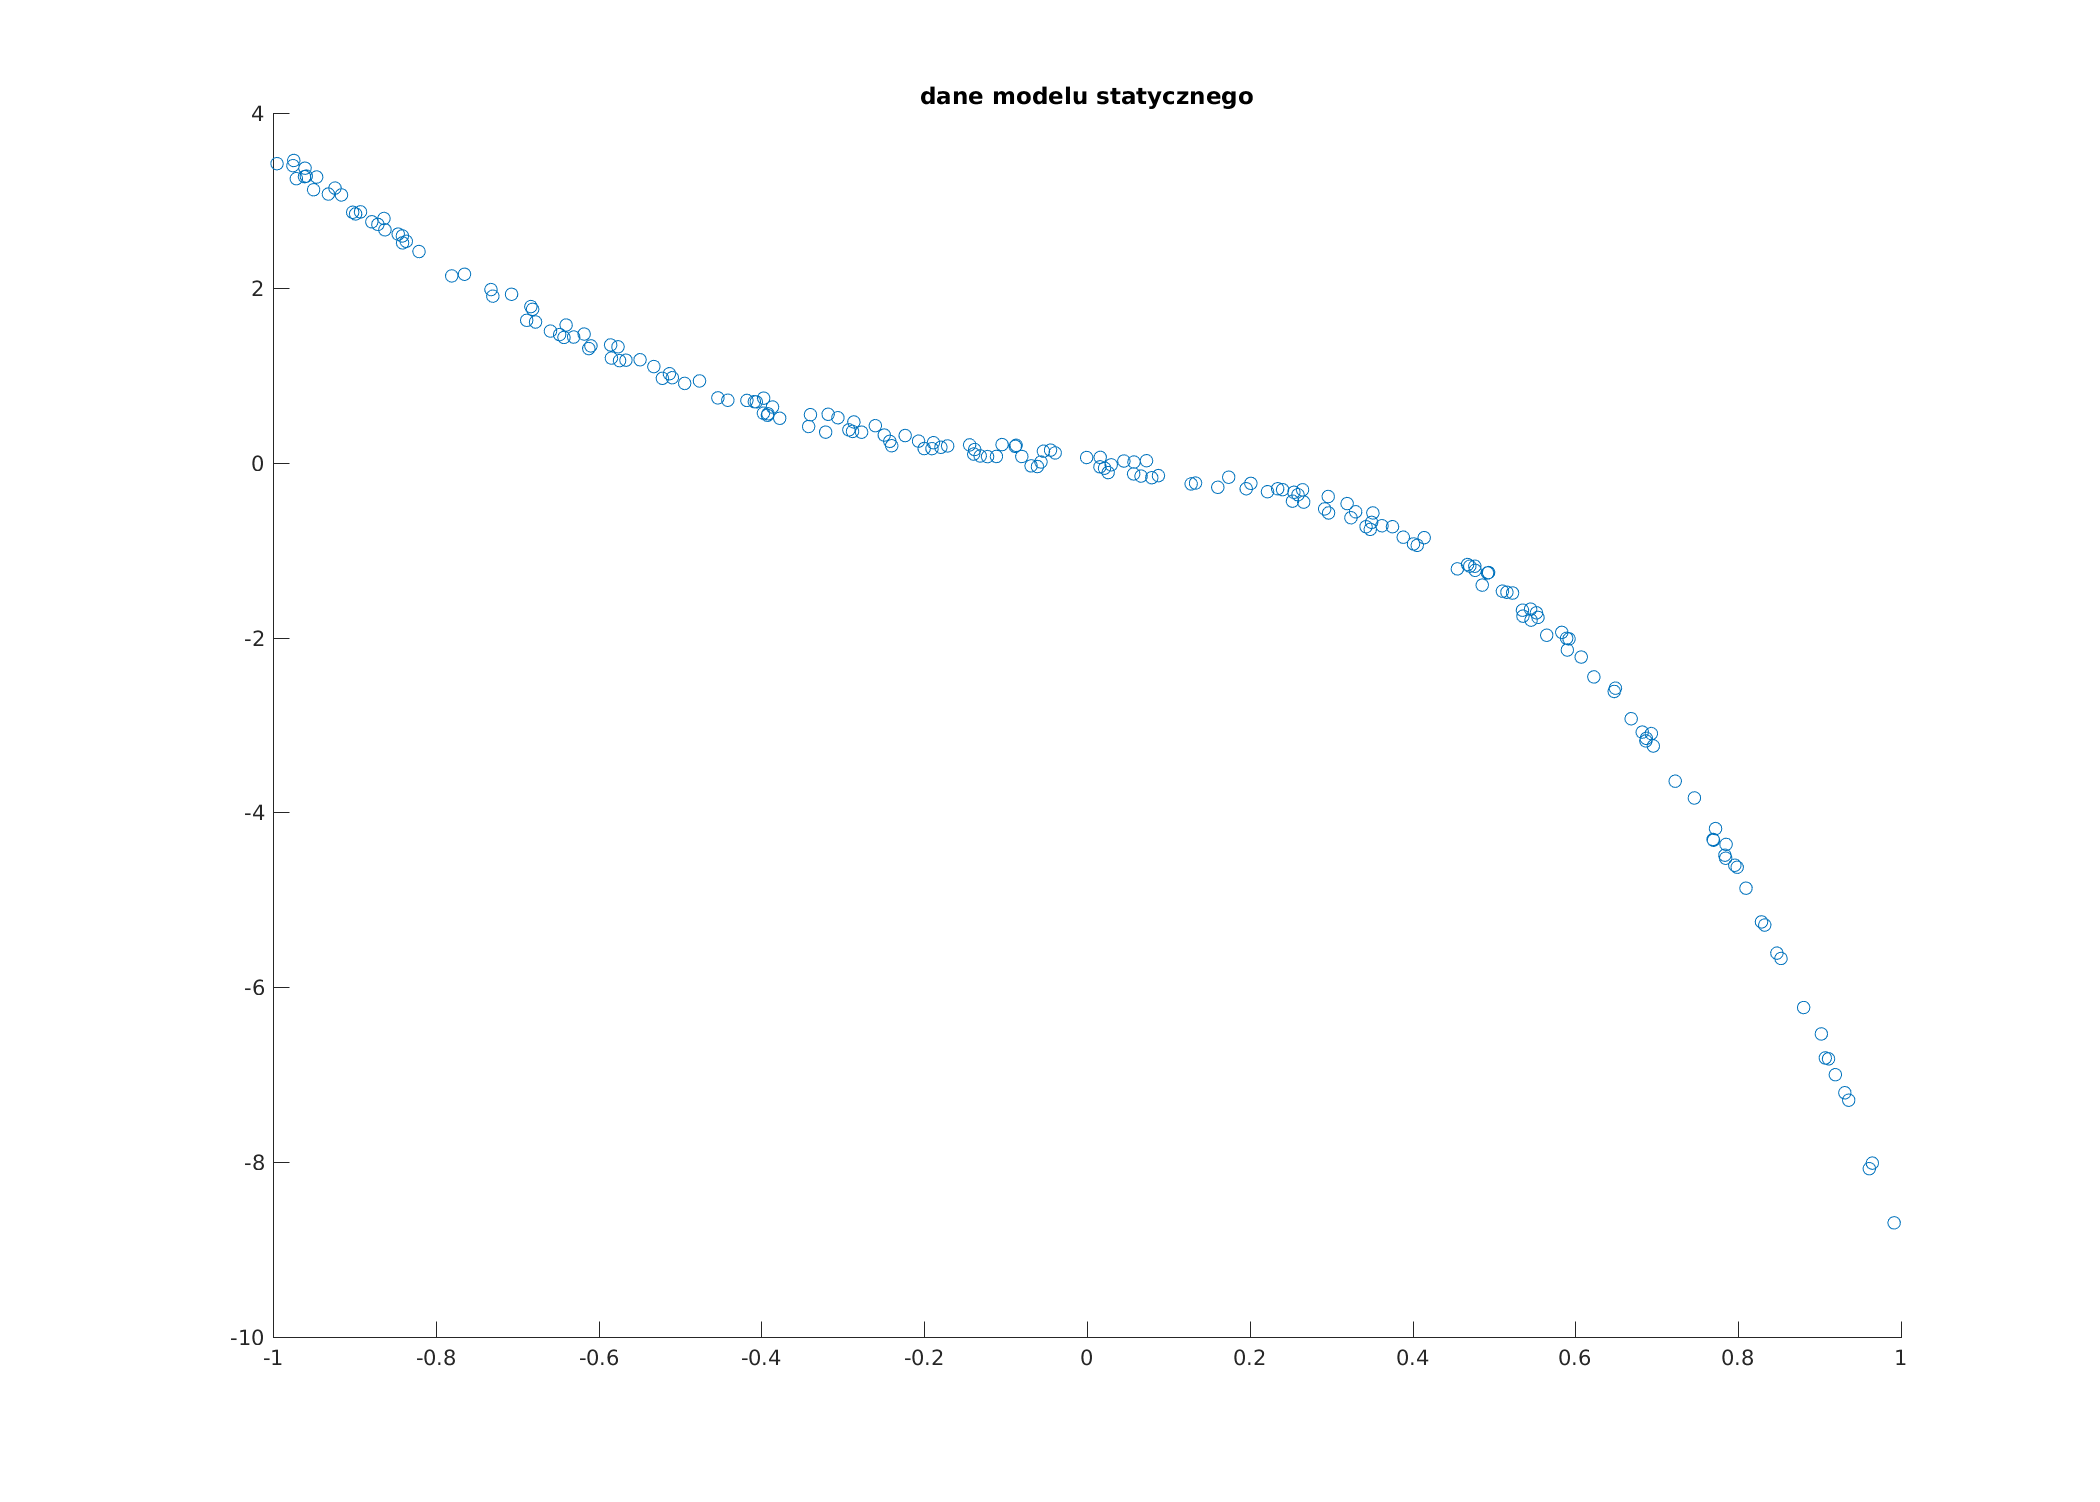
\includegraphics[scale=0.5]{dane_stat.png}
\caption{Zbiór danych statycznych}
\label{}
\end{figure}

\subsection{Podział danych statycznych na zbiory}
Dane statyczne zostały podzielone na zbiory: uczący i weryfikujący poprzez podział na parzyste i nieparzyste próbki. Dane uczące składają się z próbek parzystych, natomiast weryfikujące z próbek nieparzystych. 

\subsubsection{Reprezentacja graficzna zbioru uczącego}
\begin{figure}[H]
\centering
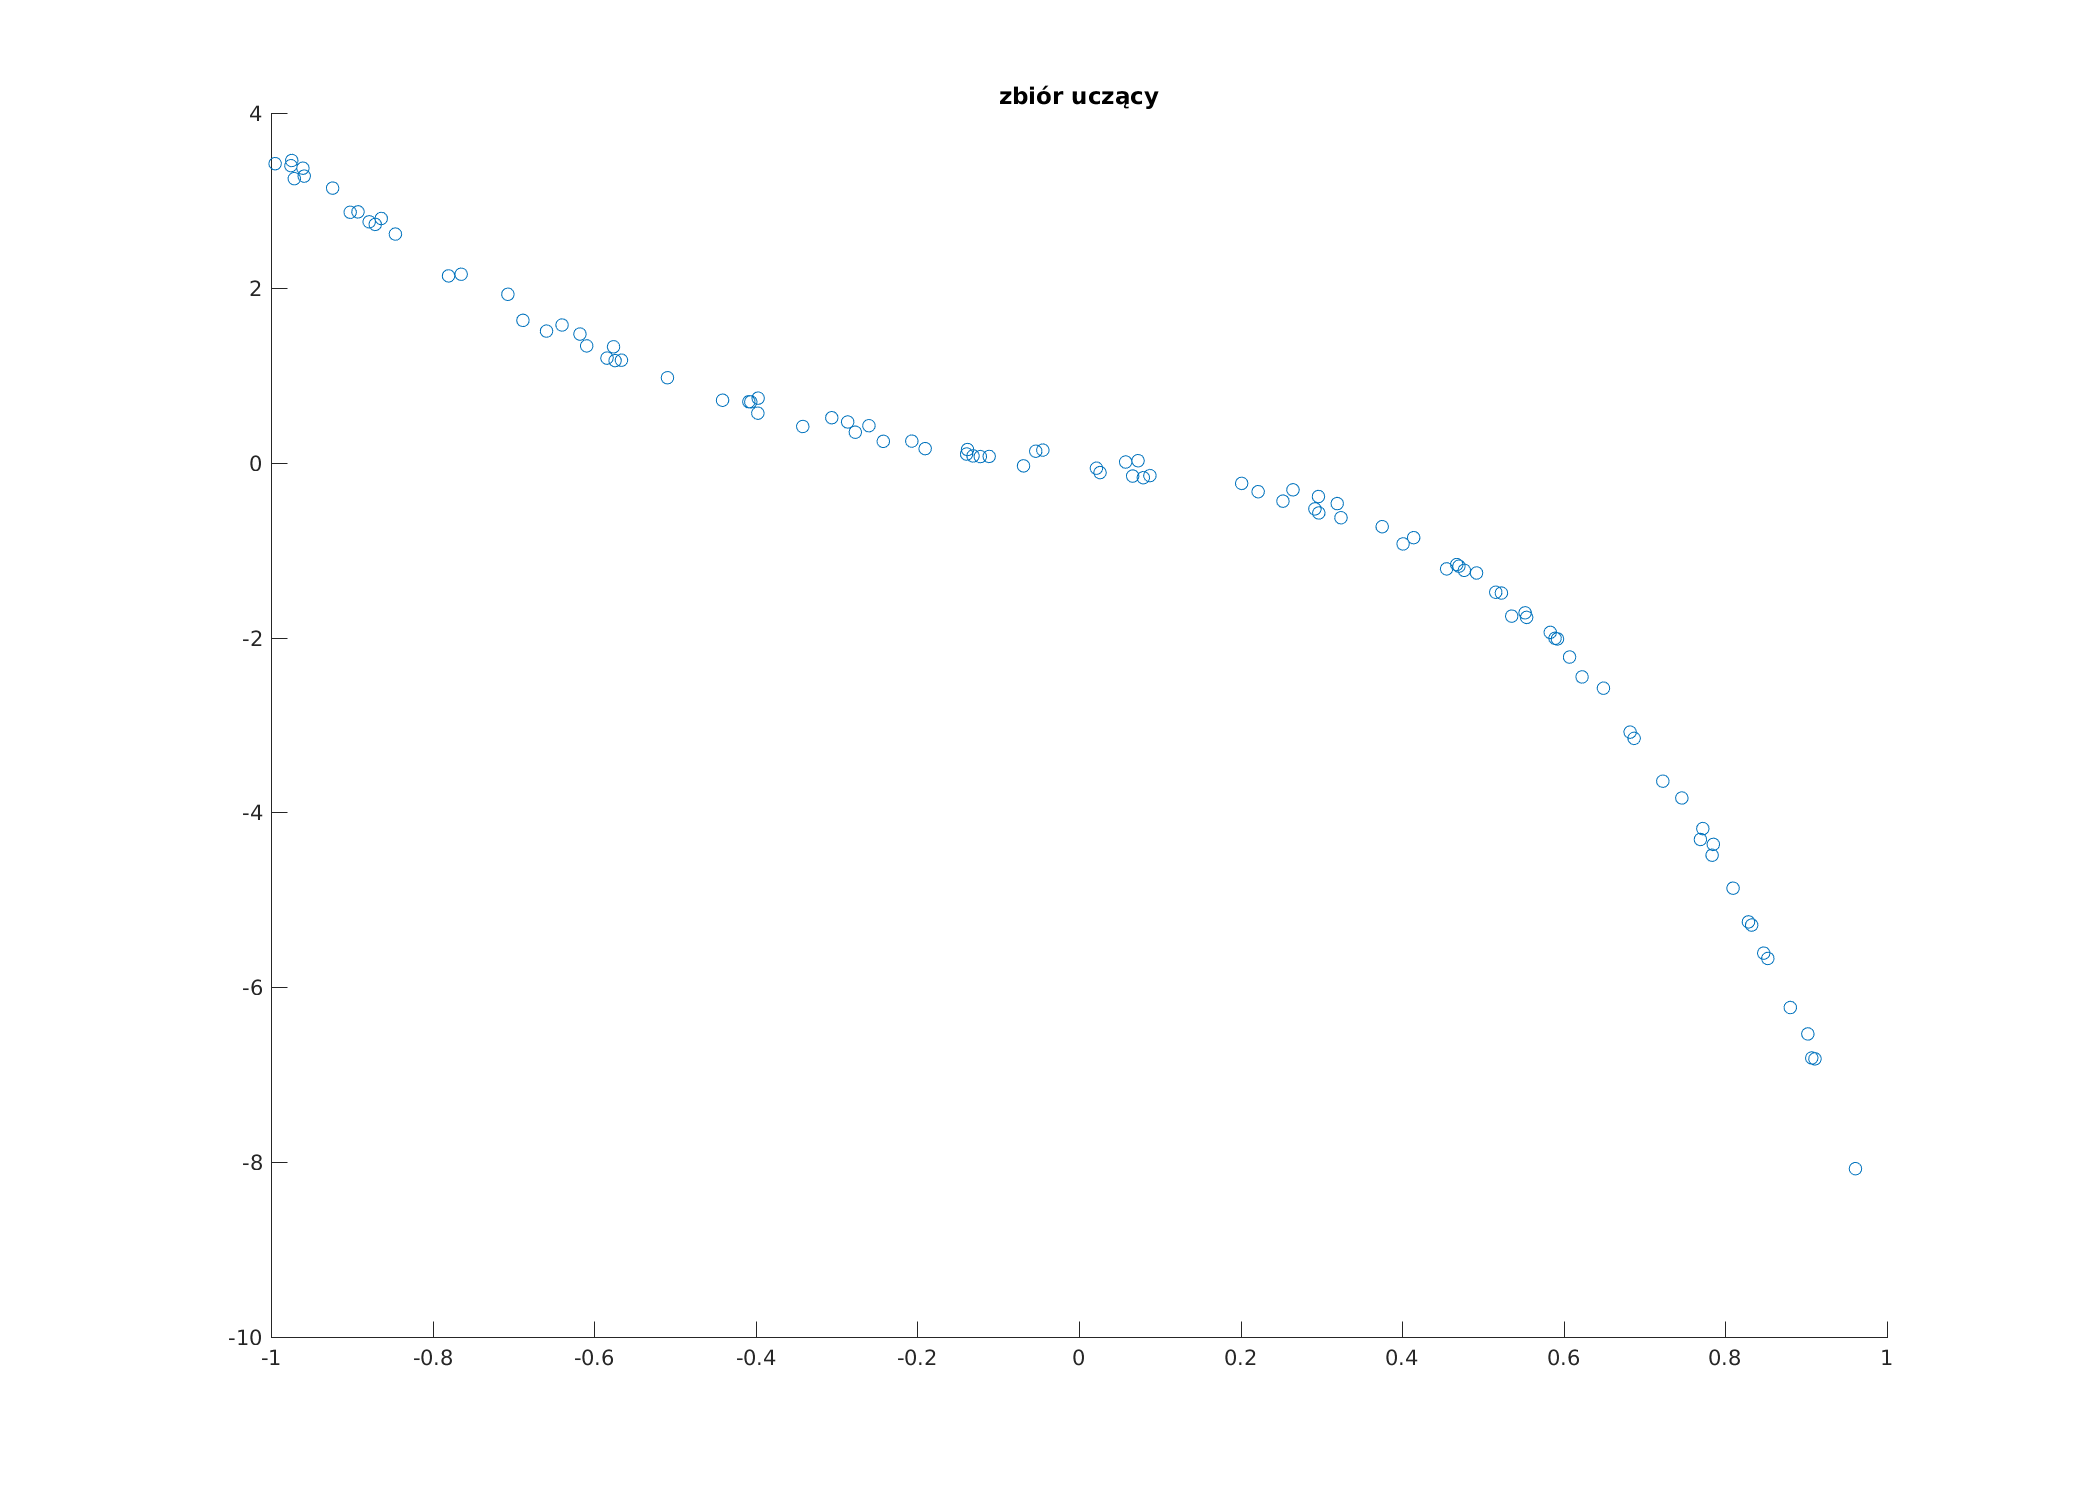
\includegraphics[scale=0.50]{dane_stat_ucz.png}
\caption{Zbiór danych uczących }
\label{}
\end{figure}

\subsubsection{Reprezentacja graficzna zbioru weryfikującego}
\begin{figure}[H]
\centering
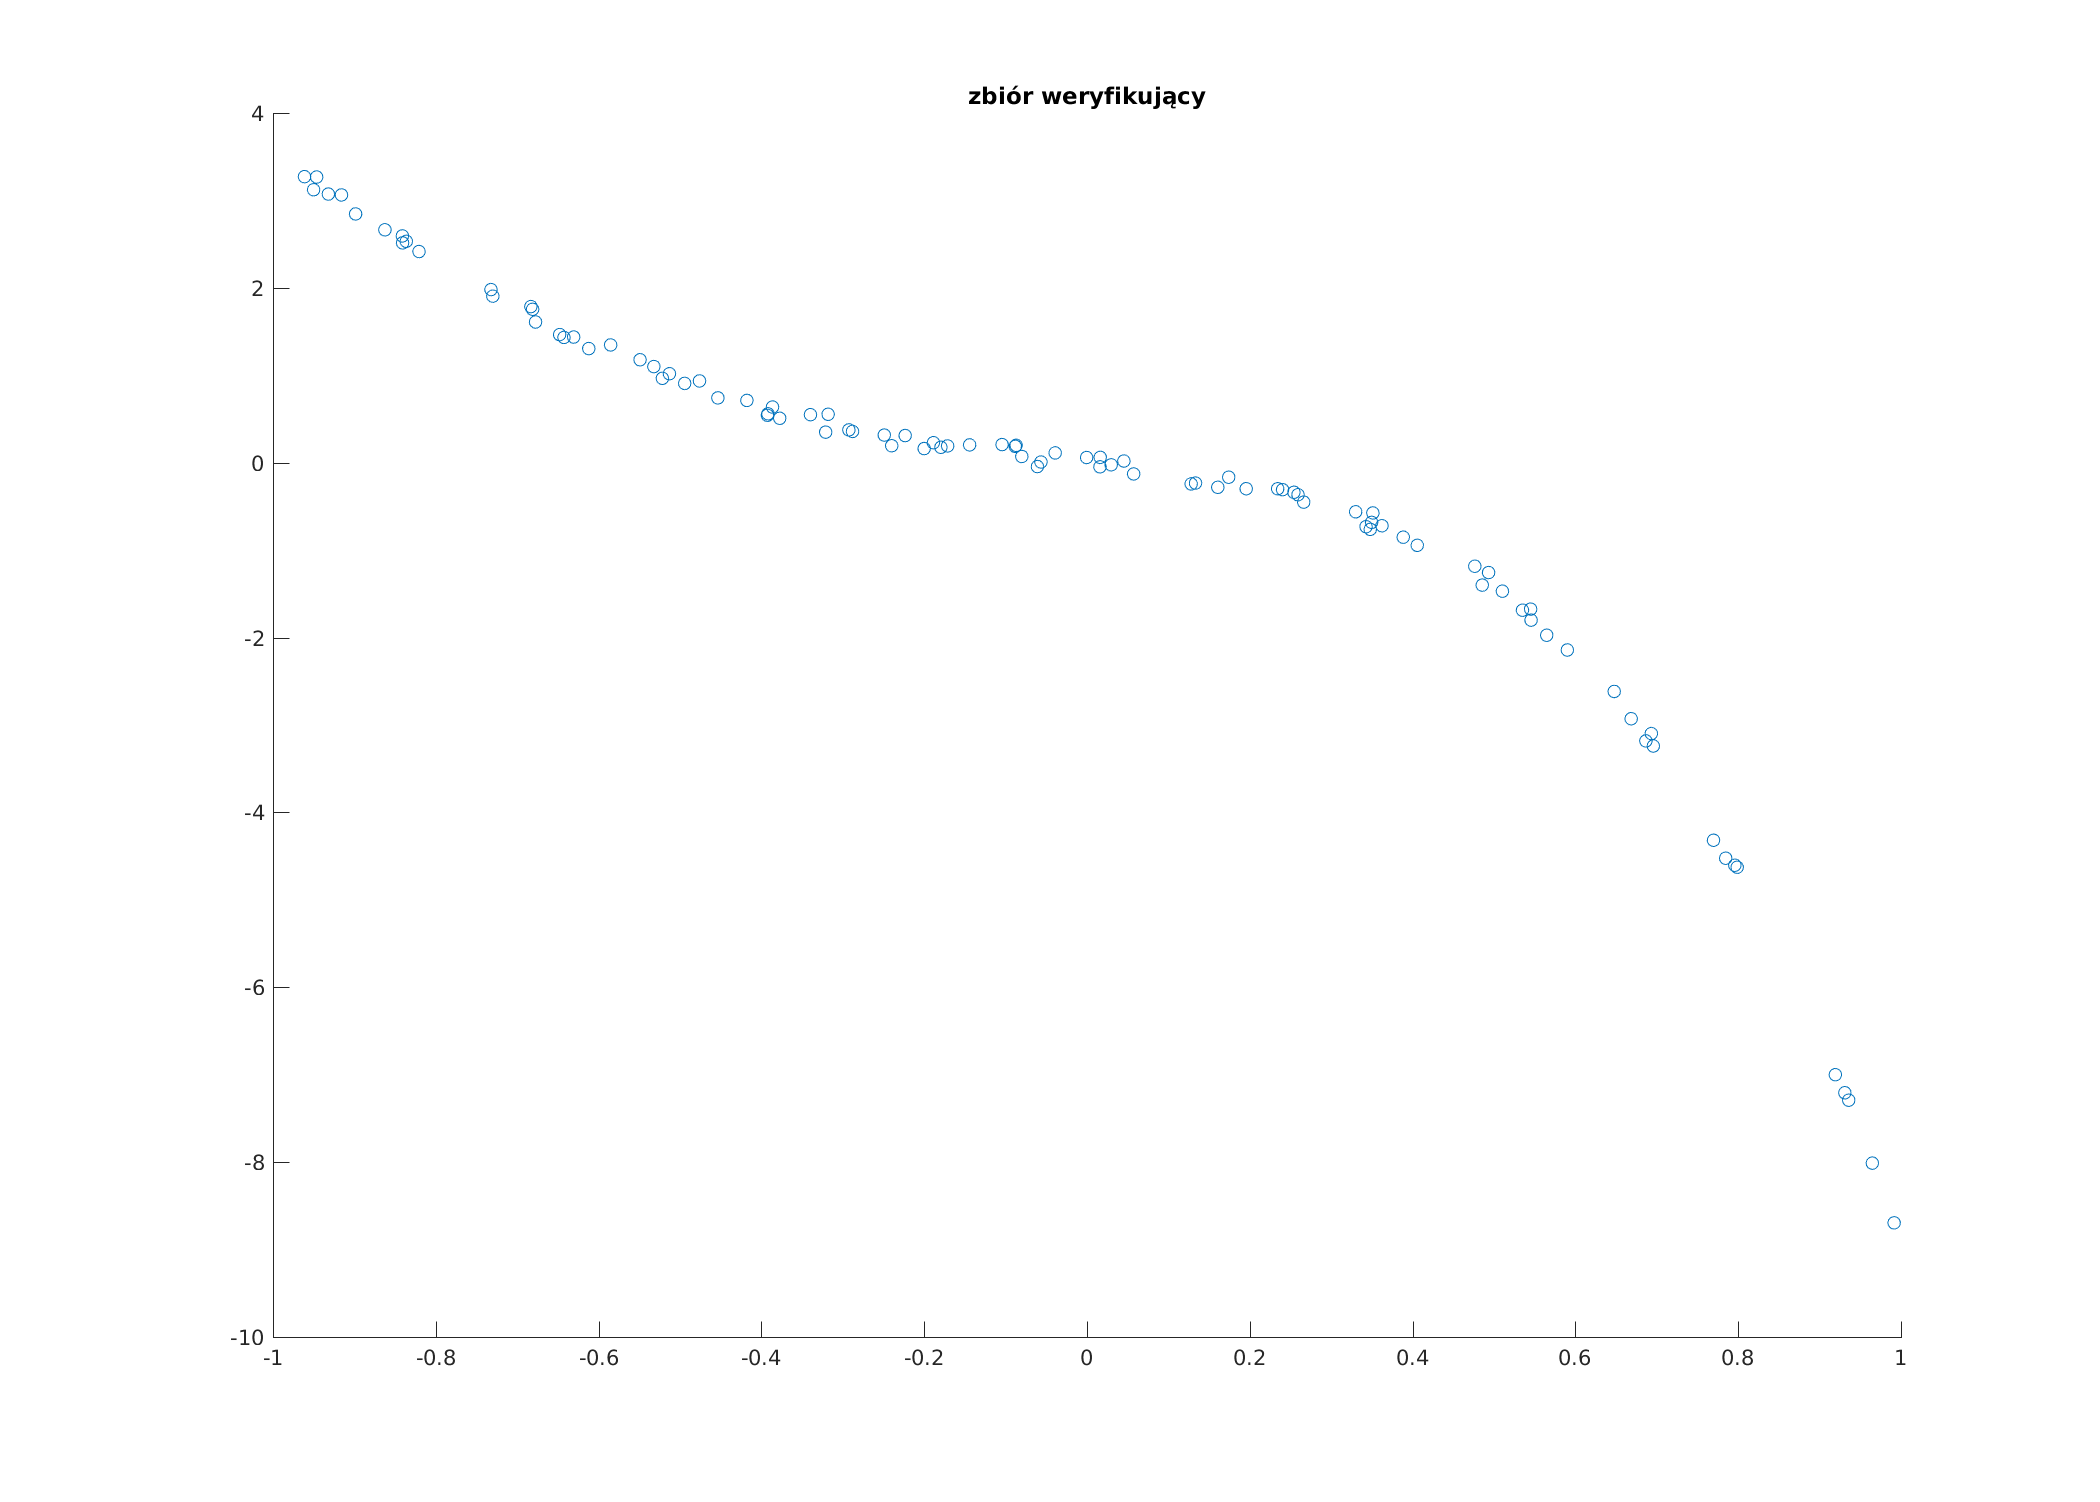
\includegraphics[scale=0.50]{dane_stat_wer.png}
\caption{Zbiór danych weryfikujących }
\label{}
\end{figure}

\subsection{Model liniowy}
Ogólna postać modelu liniowego wygląda następująco: 
$$y(u) = a_1u + a_2$$
Dla danych z zadania została wyznaczona metodą najmniejszych kwadratów i wynosi: 
$$y(u) =-4.039918564118059u -0.514971764481714  $$

\subsubsection{Wykresy charakterystyk modelu liniowego}
Poniżej znajduje się reprezentacja graficzna modelu na tle danych uczących i weryfikujących 
\subsubsection{Wykres charakterystyki na tle zbiorów danych}
\begin{figure}[H]
\centering
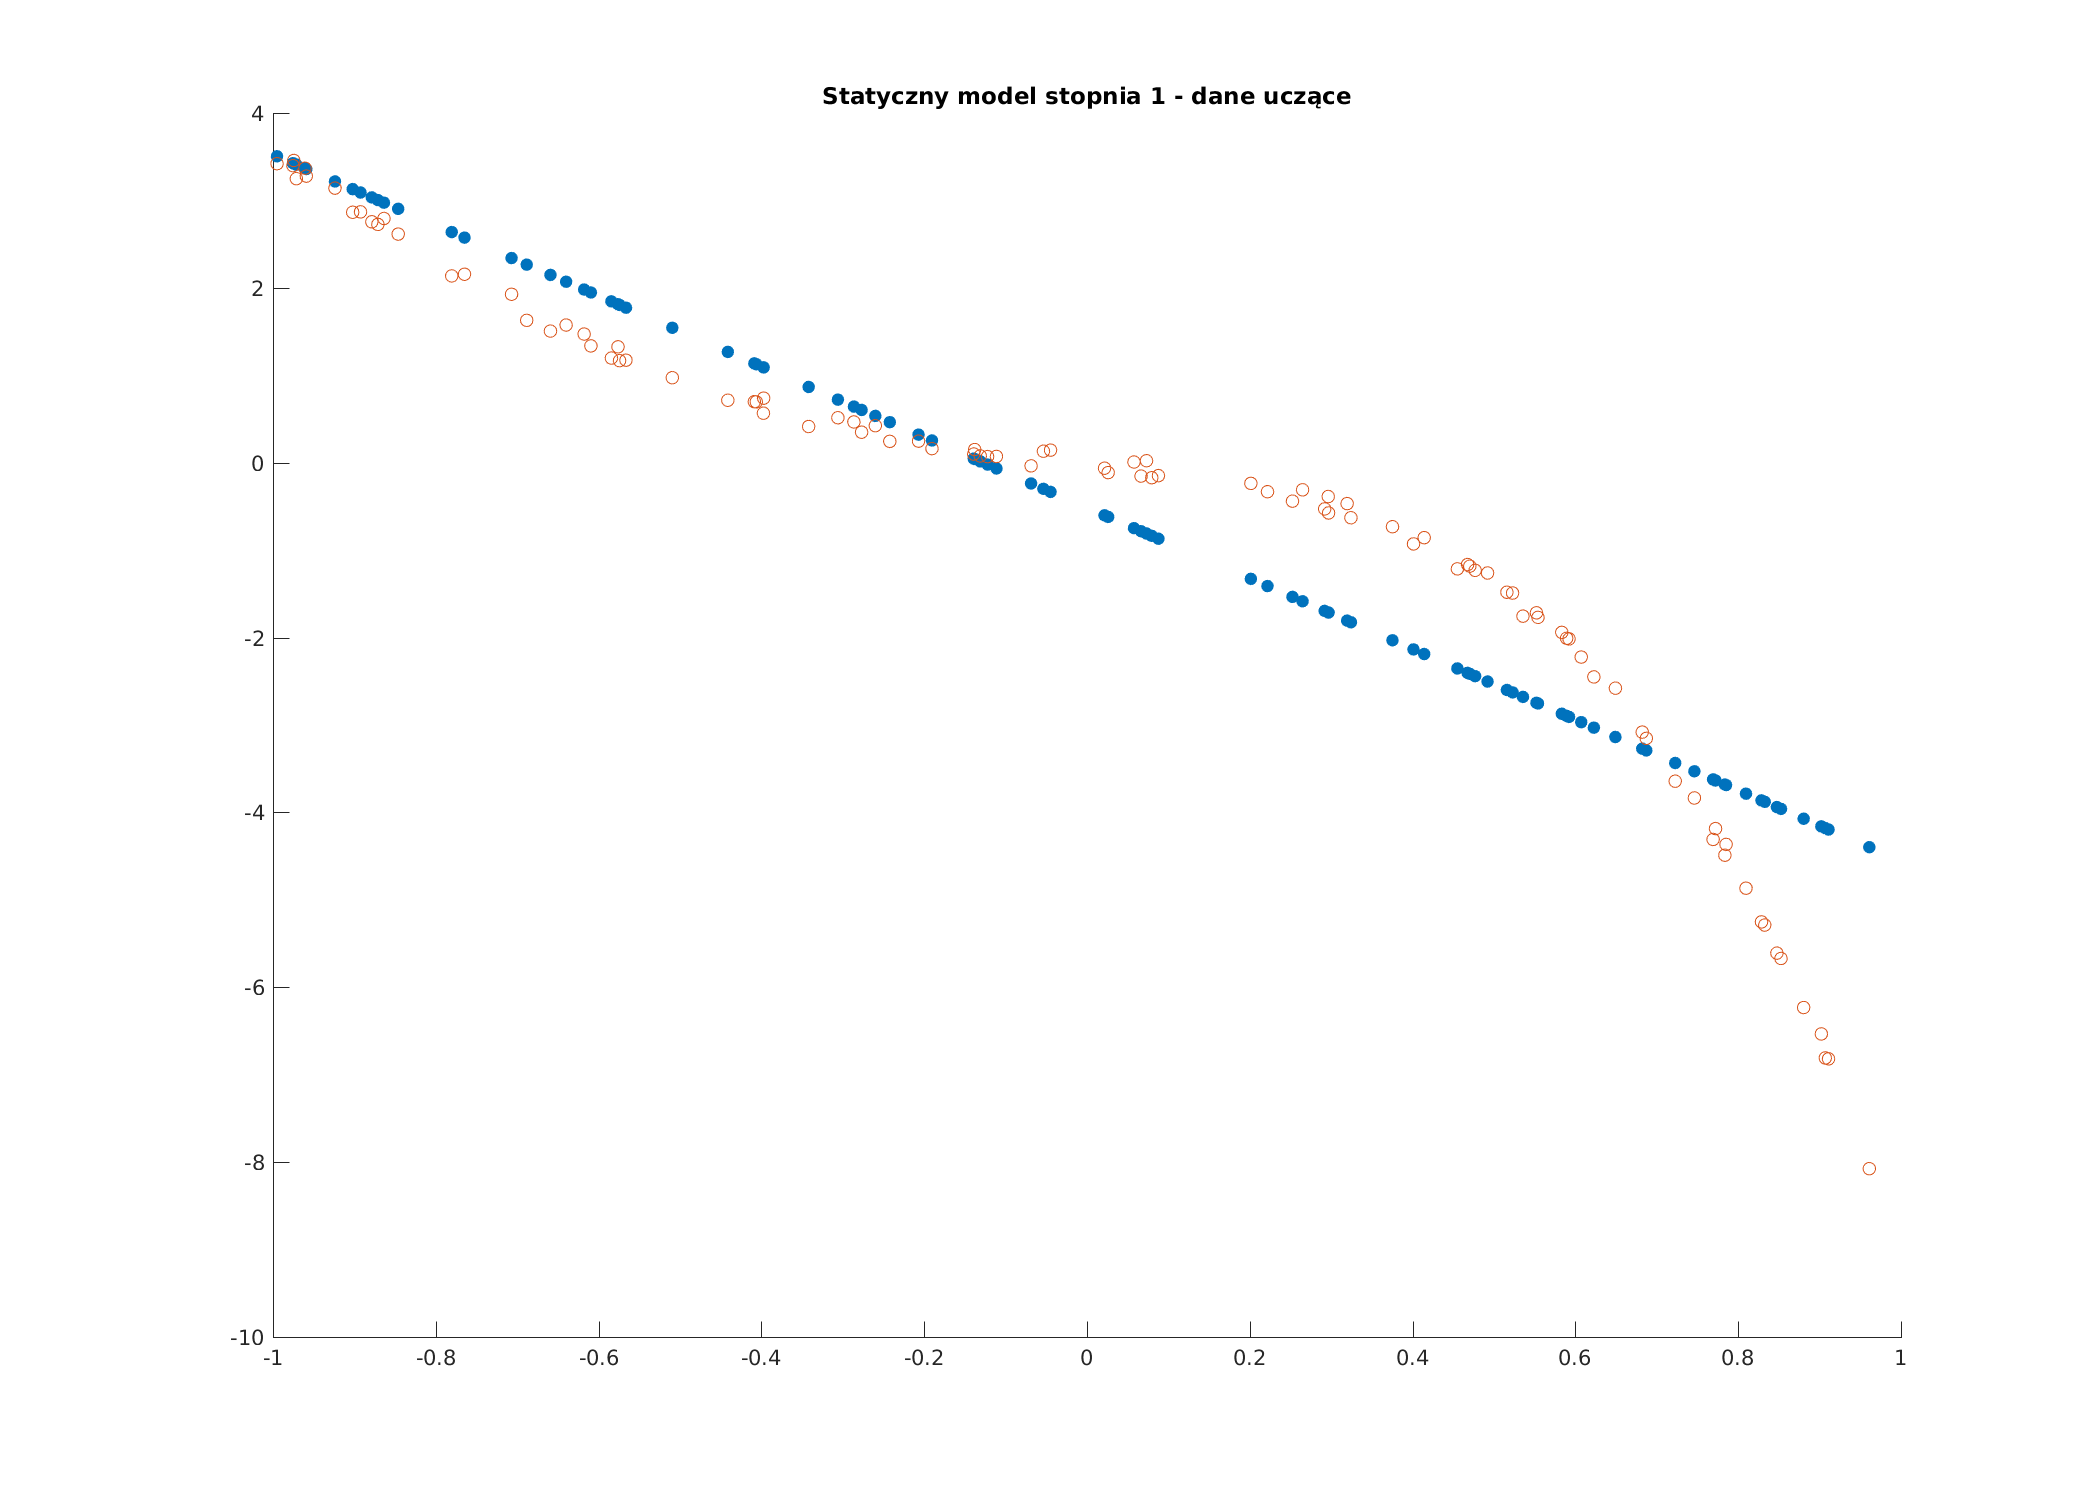
\includegraphics[scale=0.50]{dane_stat_1_ucz.png}
\caption{Charakterystyka modelu na tle zbioru danych uczących}
\label{}
\end{figure}
\begin{figure}[H]
\centering
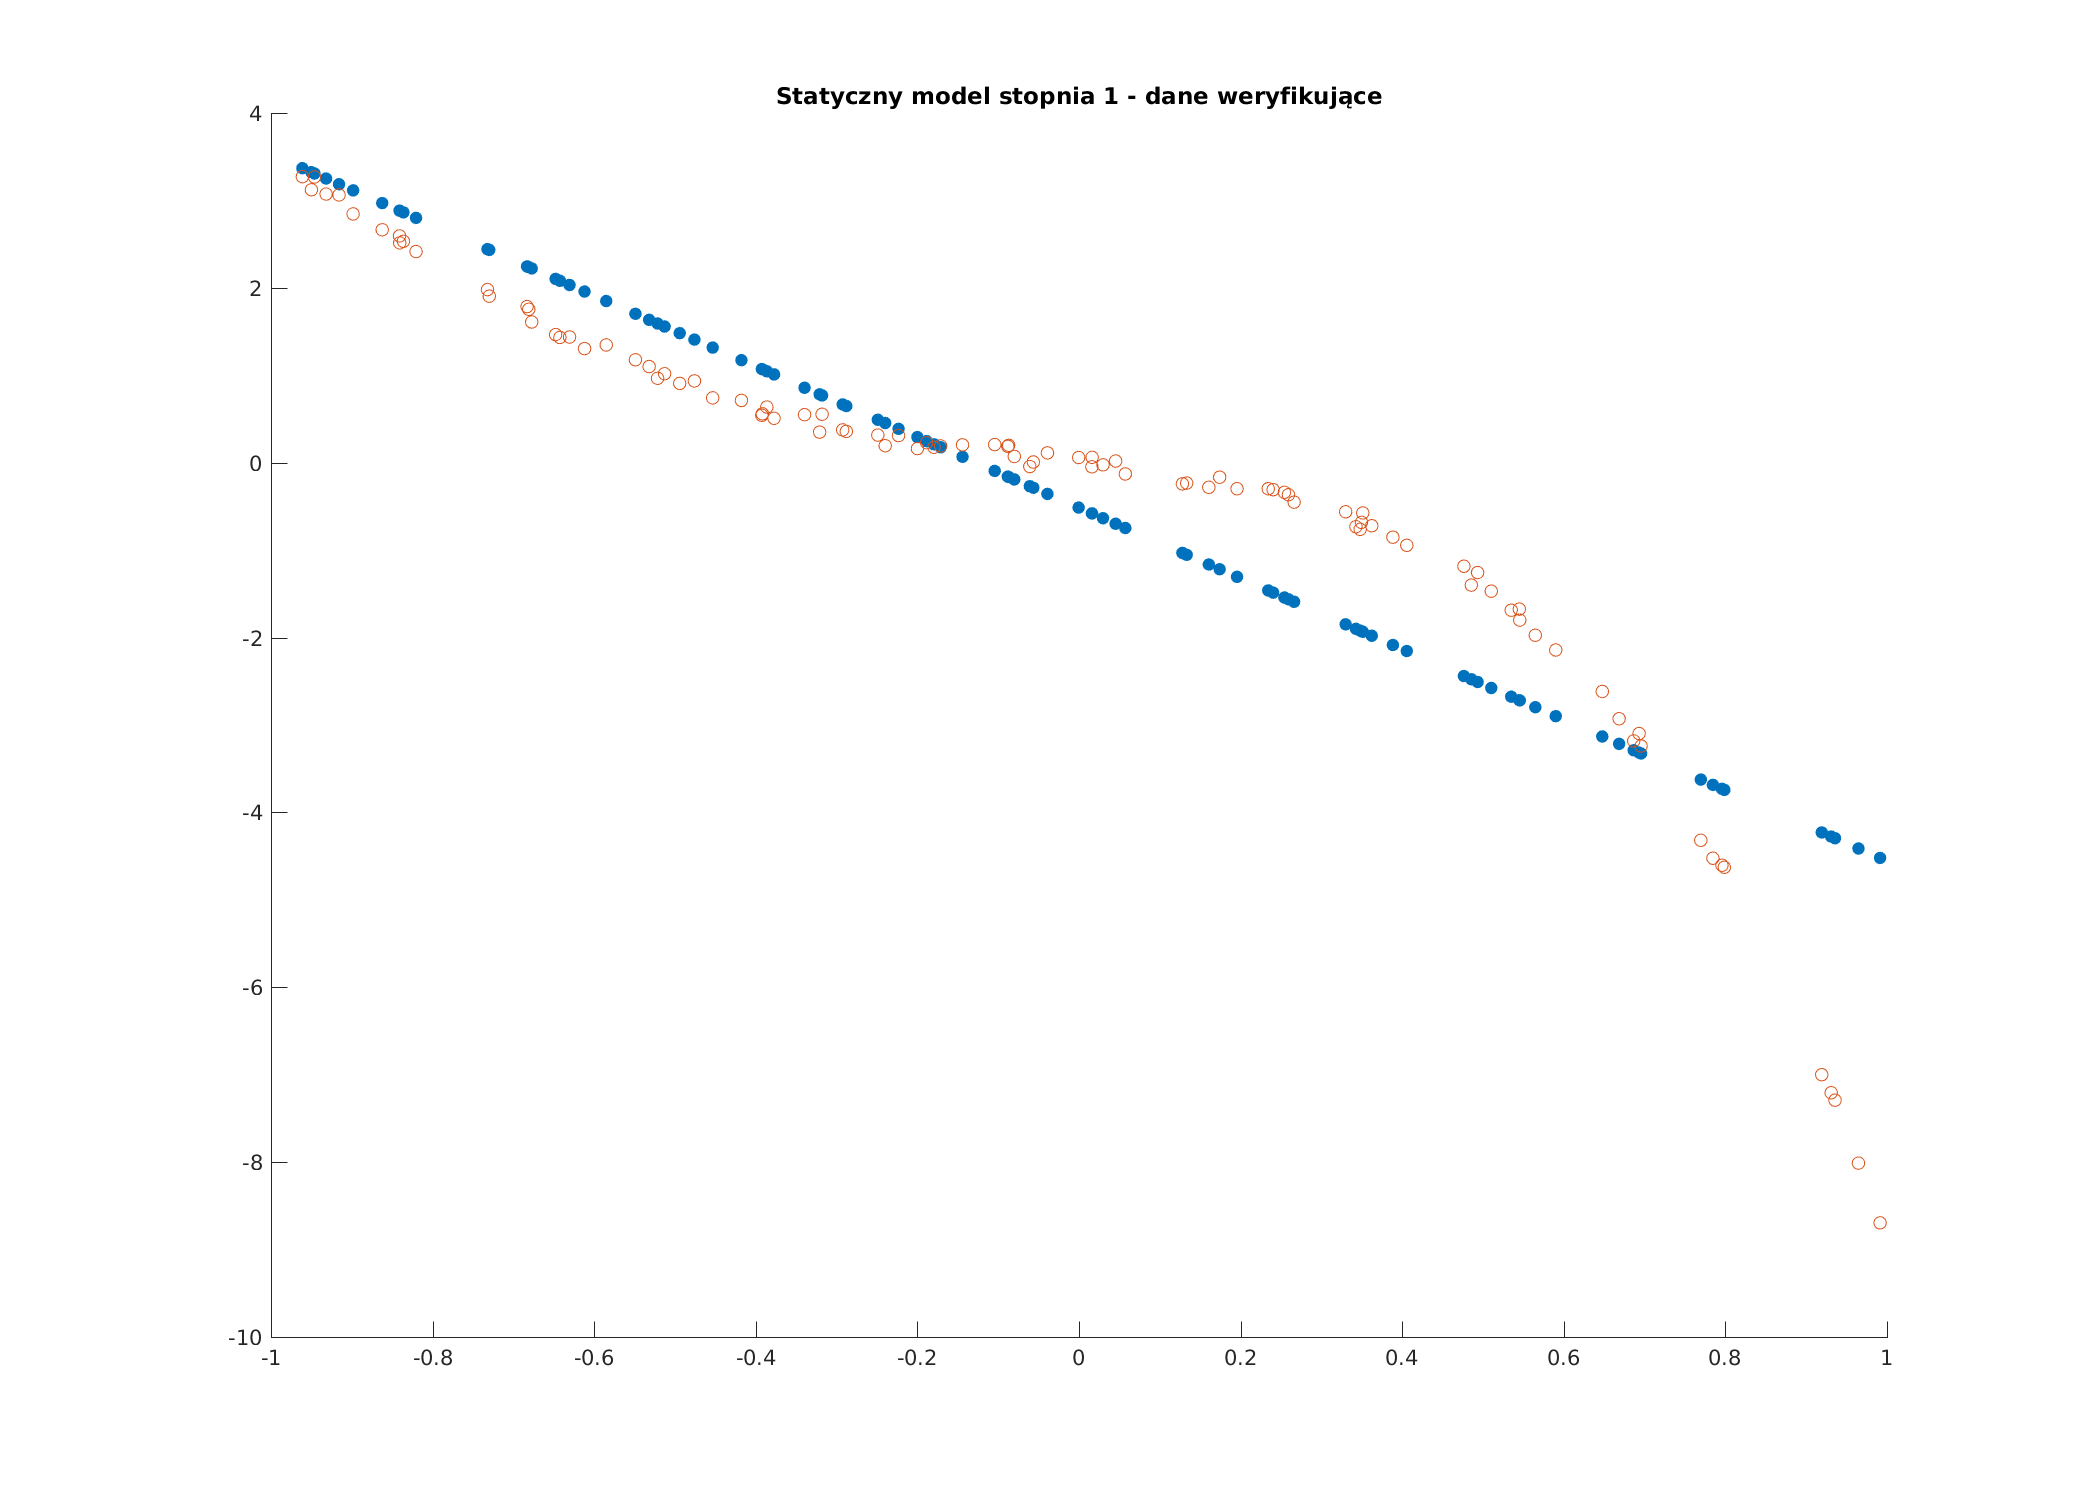
\includegraphics[scale=0.50]{dane_stat_1_wer.png}
\caption{Charakterystyka modelu na tle zbioru danych weryfikujących }
\label{}
\end{figure}


\subsubsection{Błędy zbiorów}
\begin{figure}[H]
\centering
\begin{tabular}{|c|c|c|}
\hline
	N & Błąd dla danych uczących & Błąd dla danych weryfikujących\\
\hline
	1 & 9.432614 & 1.028\\
\hline
\end{tabular}
\caption{Błędy modelu liniowego}
\end{figure}


\subsection{Statyczne modele nieliniowe}
Dla danych z zadania model nielinowy mało dokładnie odwzorowuje poszczególne próbki, dlatego kolejnym krokiem jest wyznaczenie modeli wyższego stopnia. 

\subsubsection{Model stopnia drugiego}
\begin{figure}[H]
\centering
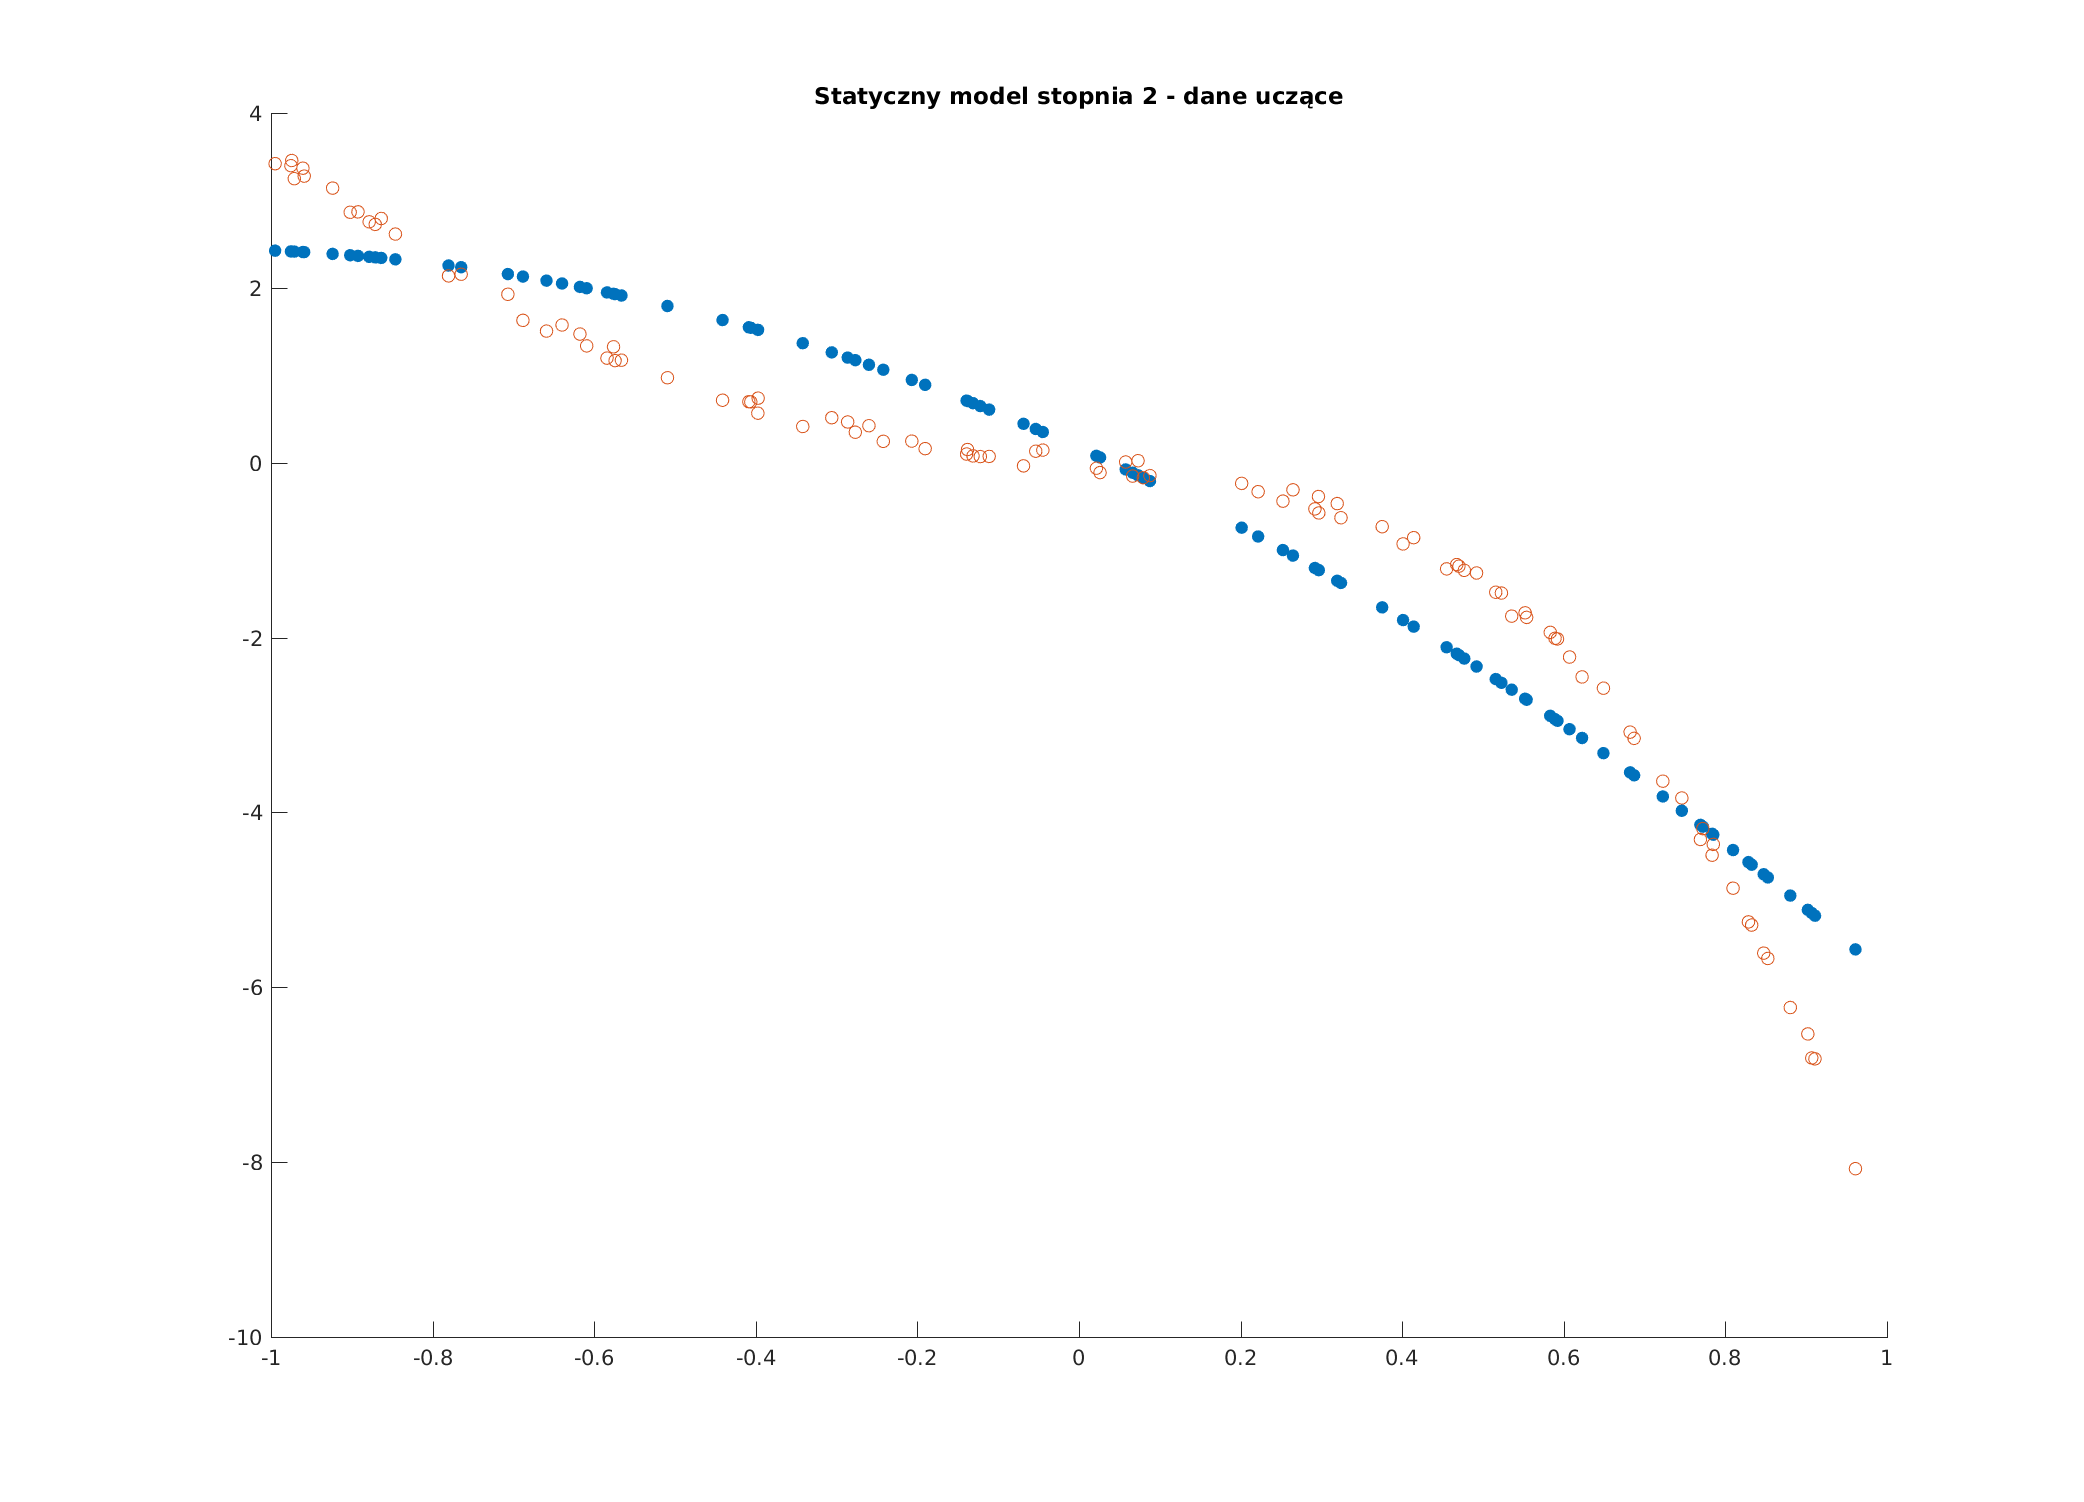
\includegraphics[scale=0.50]{dane_stat_2_ucz.png}
\caption{Model stopnia drugiego dane uczące}
\label{}
\end{figure}

\begin{figure}[H]
\centering
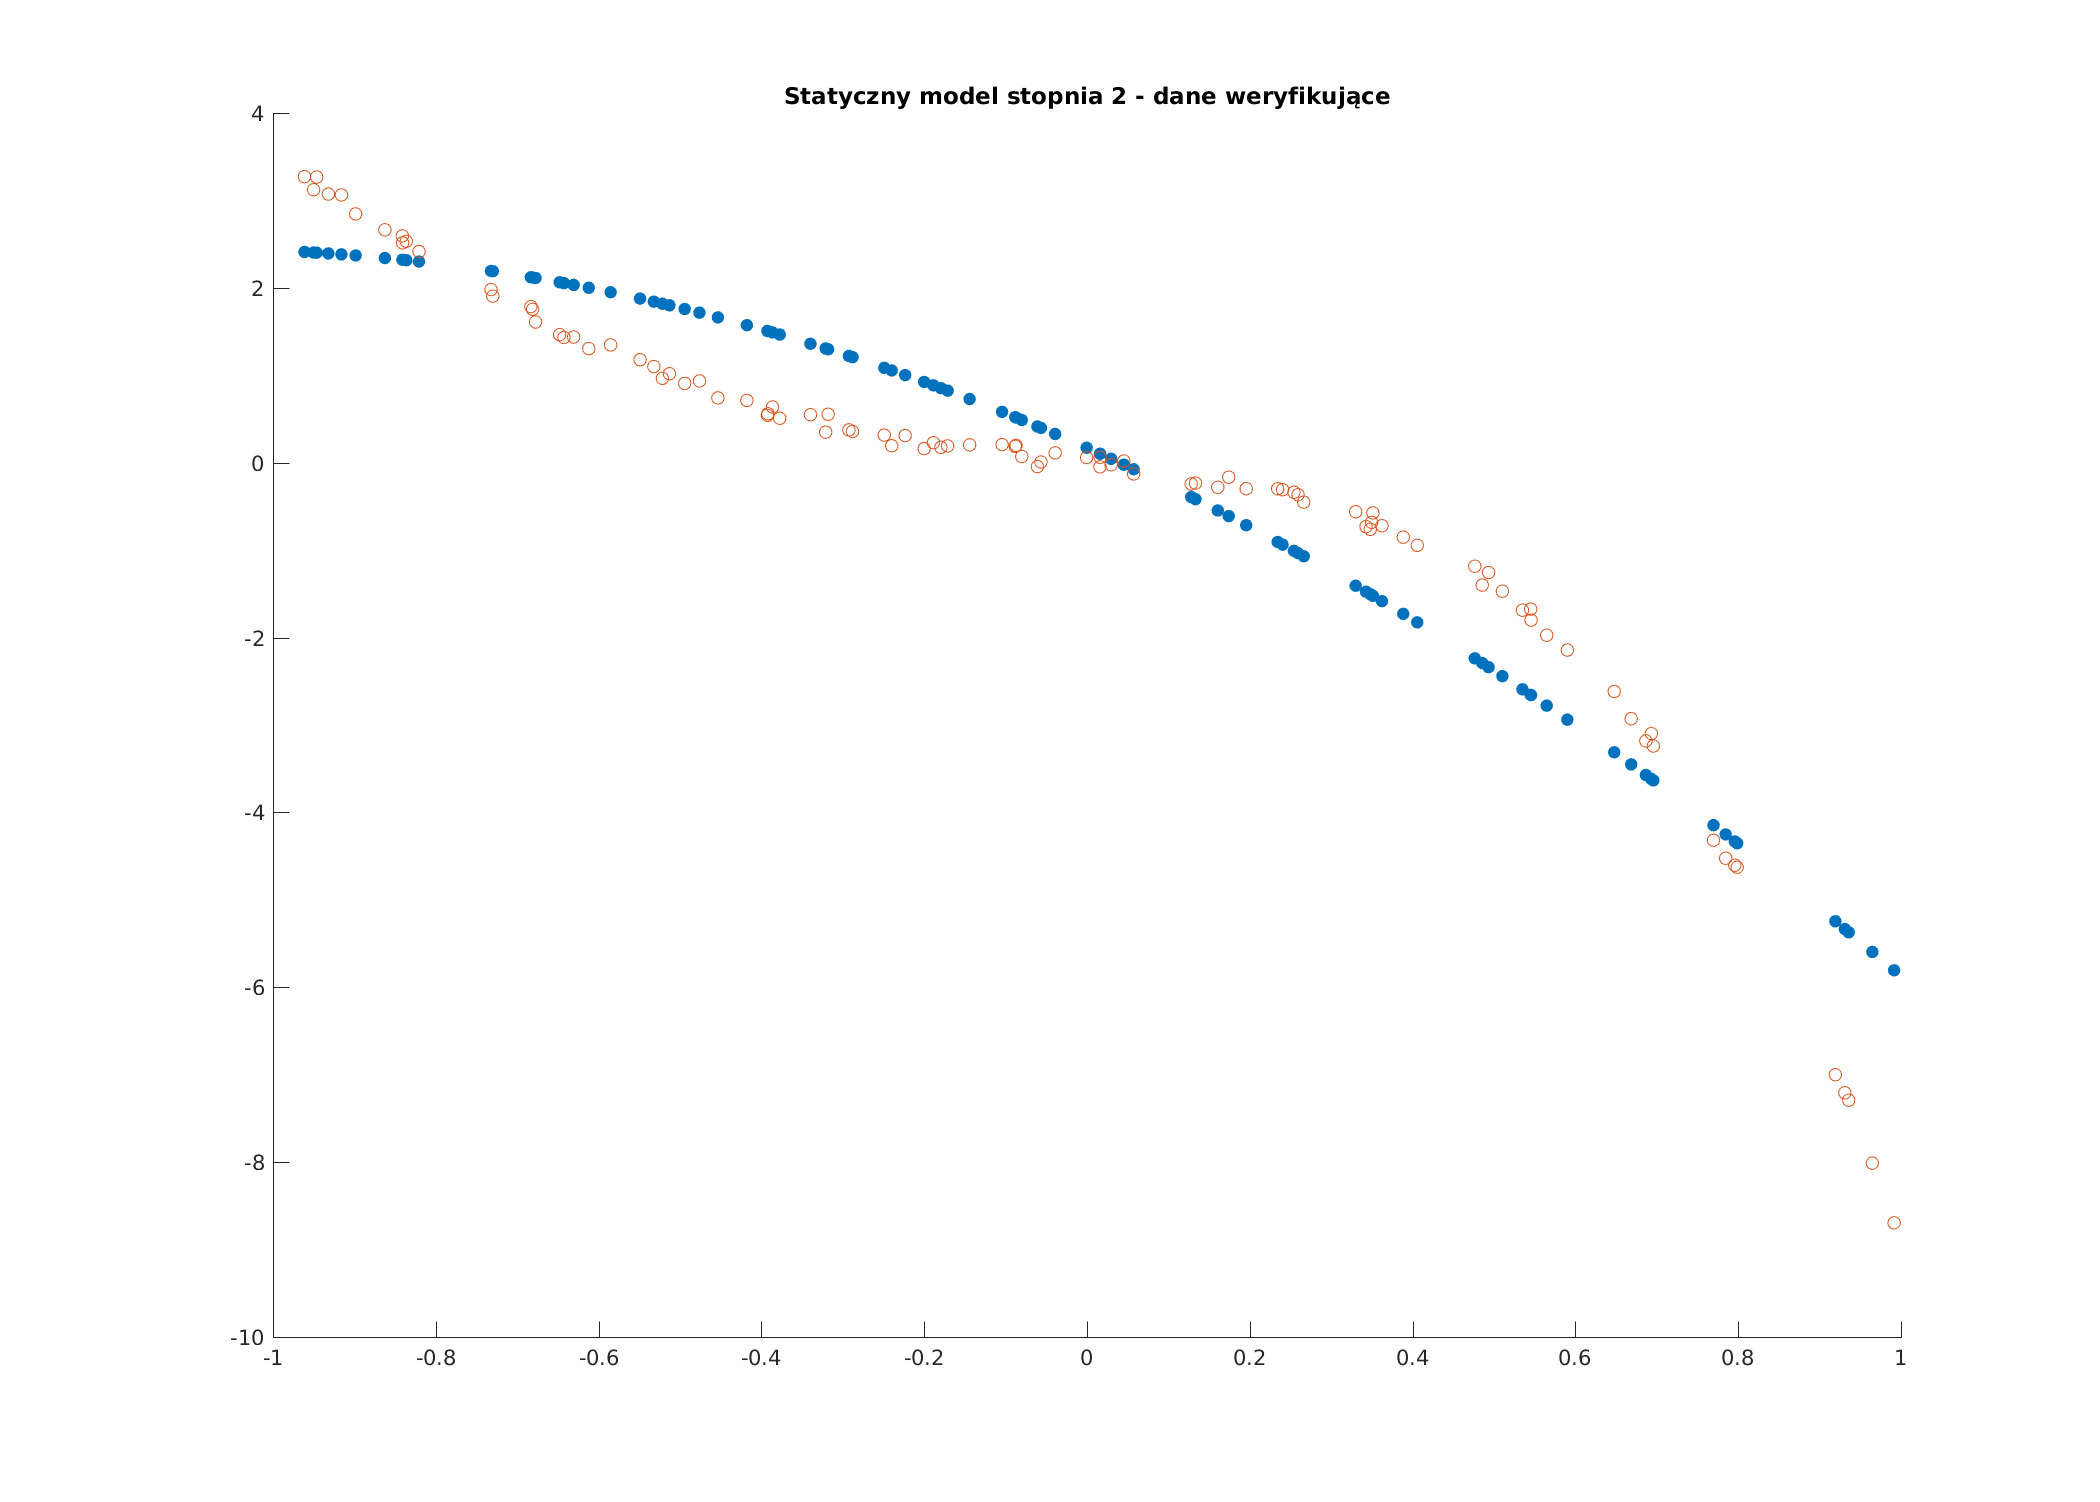
\includegraphics[scale=0.50]{dane_stat_2_wer.png}
\caption{Model stopnia drugiego dane weryfikujące}
\label{}
\end{figure}

\subsubsection{Model stopnia trzeciego}
\begin{figure}[H]
\centering
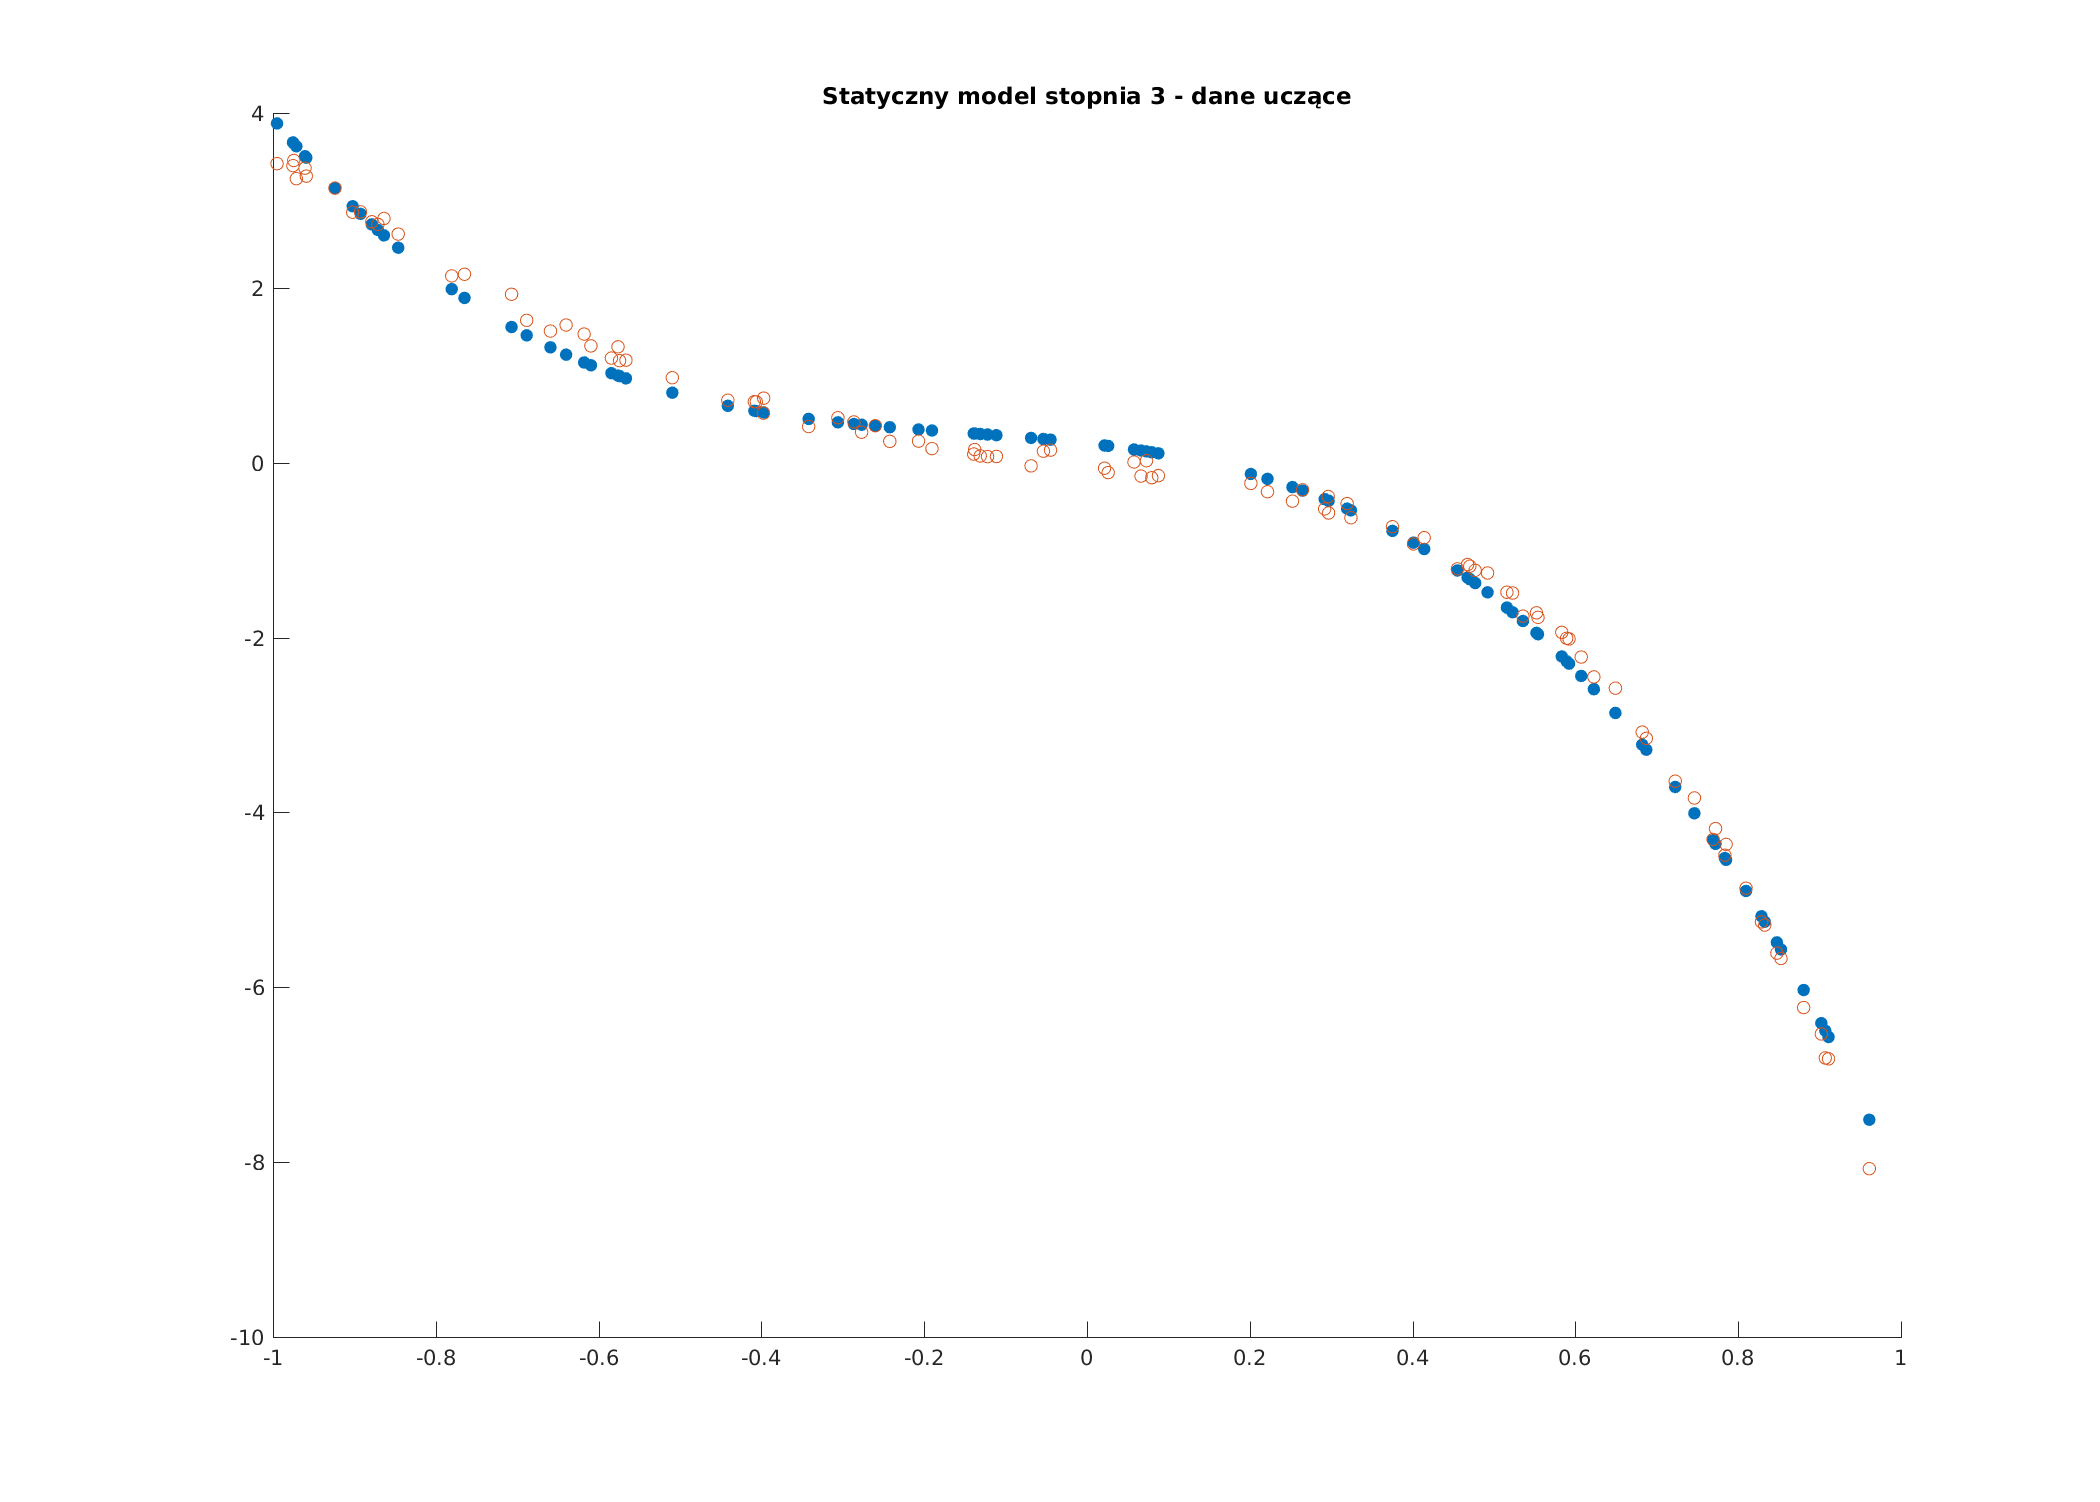
\includegraphics[scale=0.50]{dane_stat_3_ucz.png}
\caption{Model stopnia trzeciego dane uczące}
\label{}
\end{figure}

\begin{figure}[H]
\centering
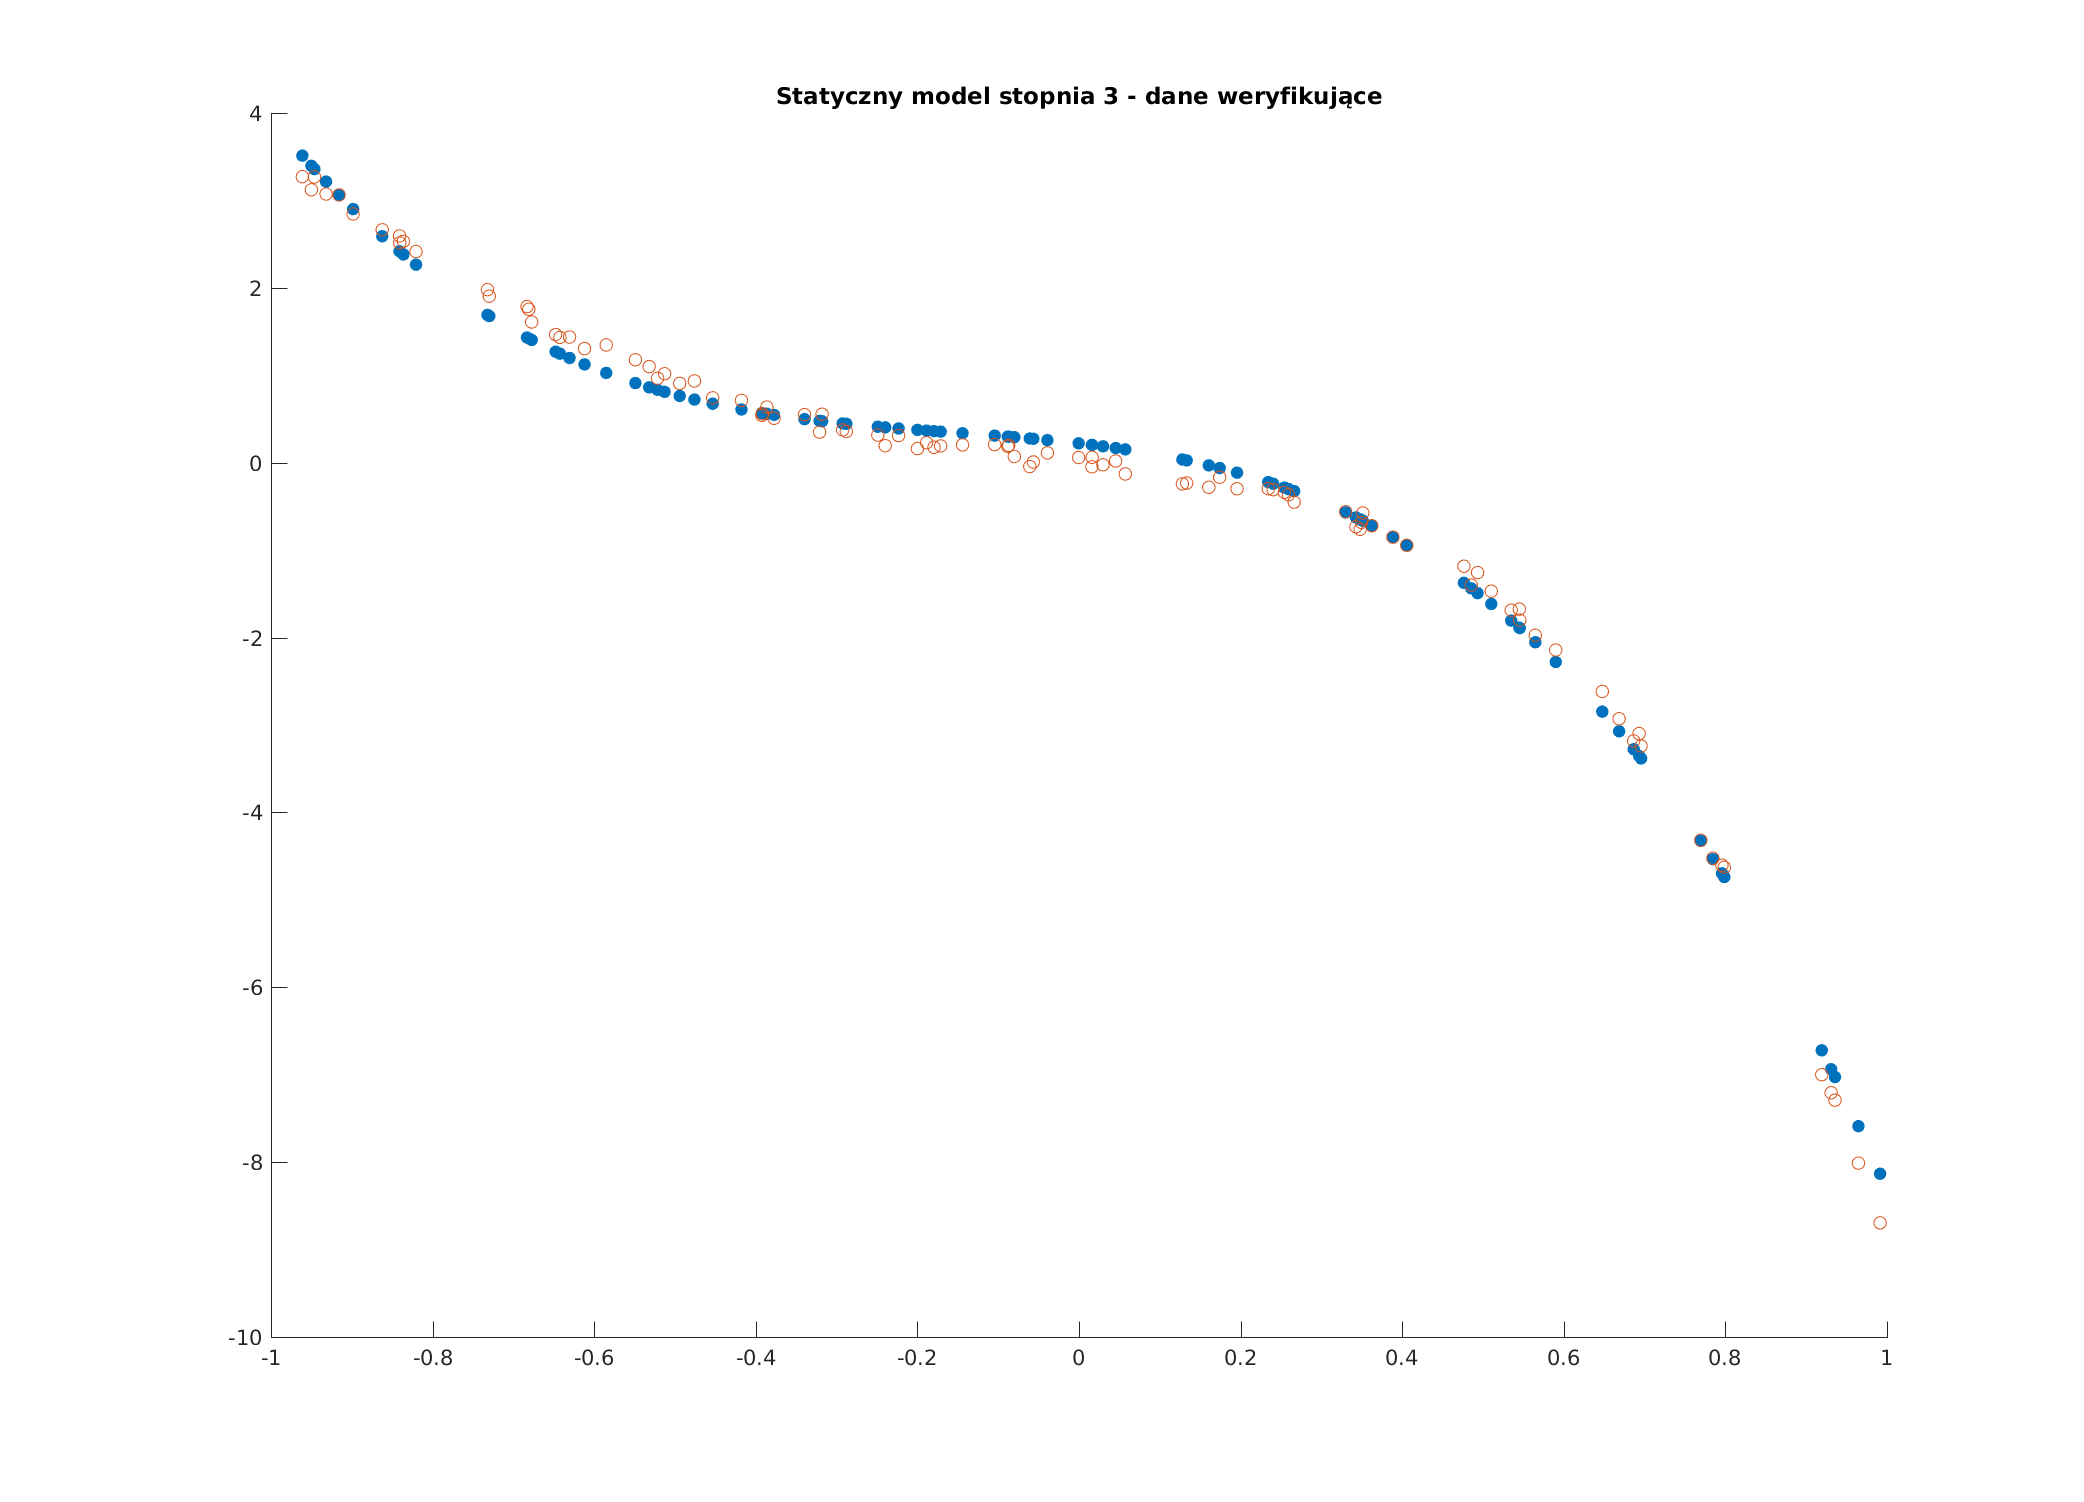
\includegraphics[scale=0.50]{dane_stat_3_wer.png}
\caption{Model stopnia trzeciego dane weryfikujące}
\label{}
\end{figure}

\subsubsection{Model stopnia czwartego}
\begin{figure}[H]
\centering
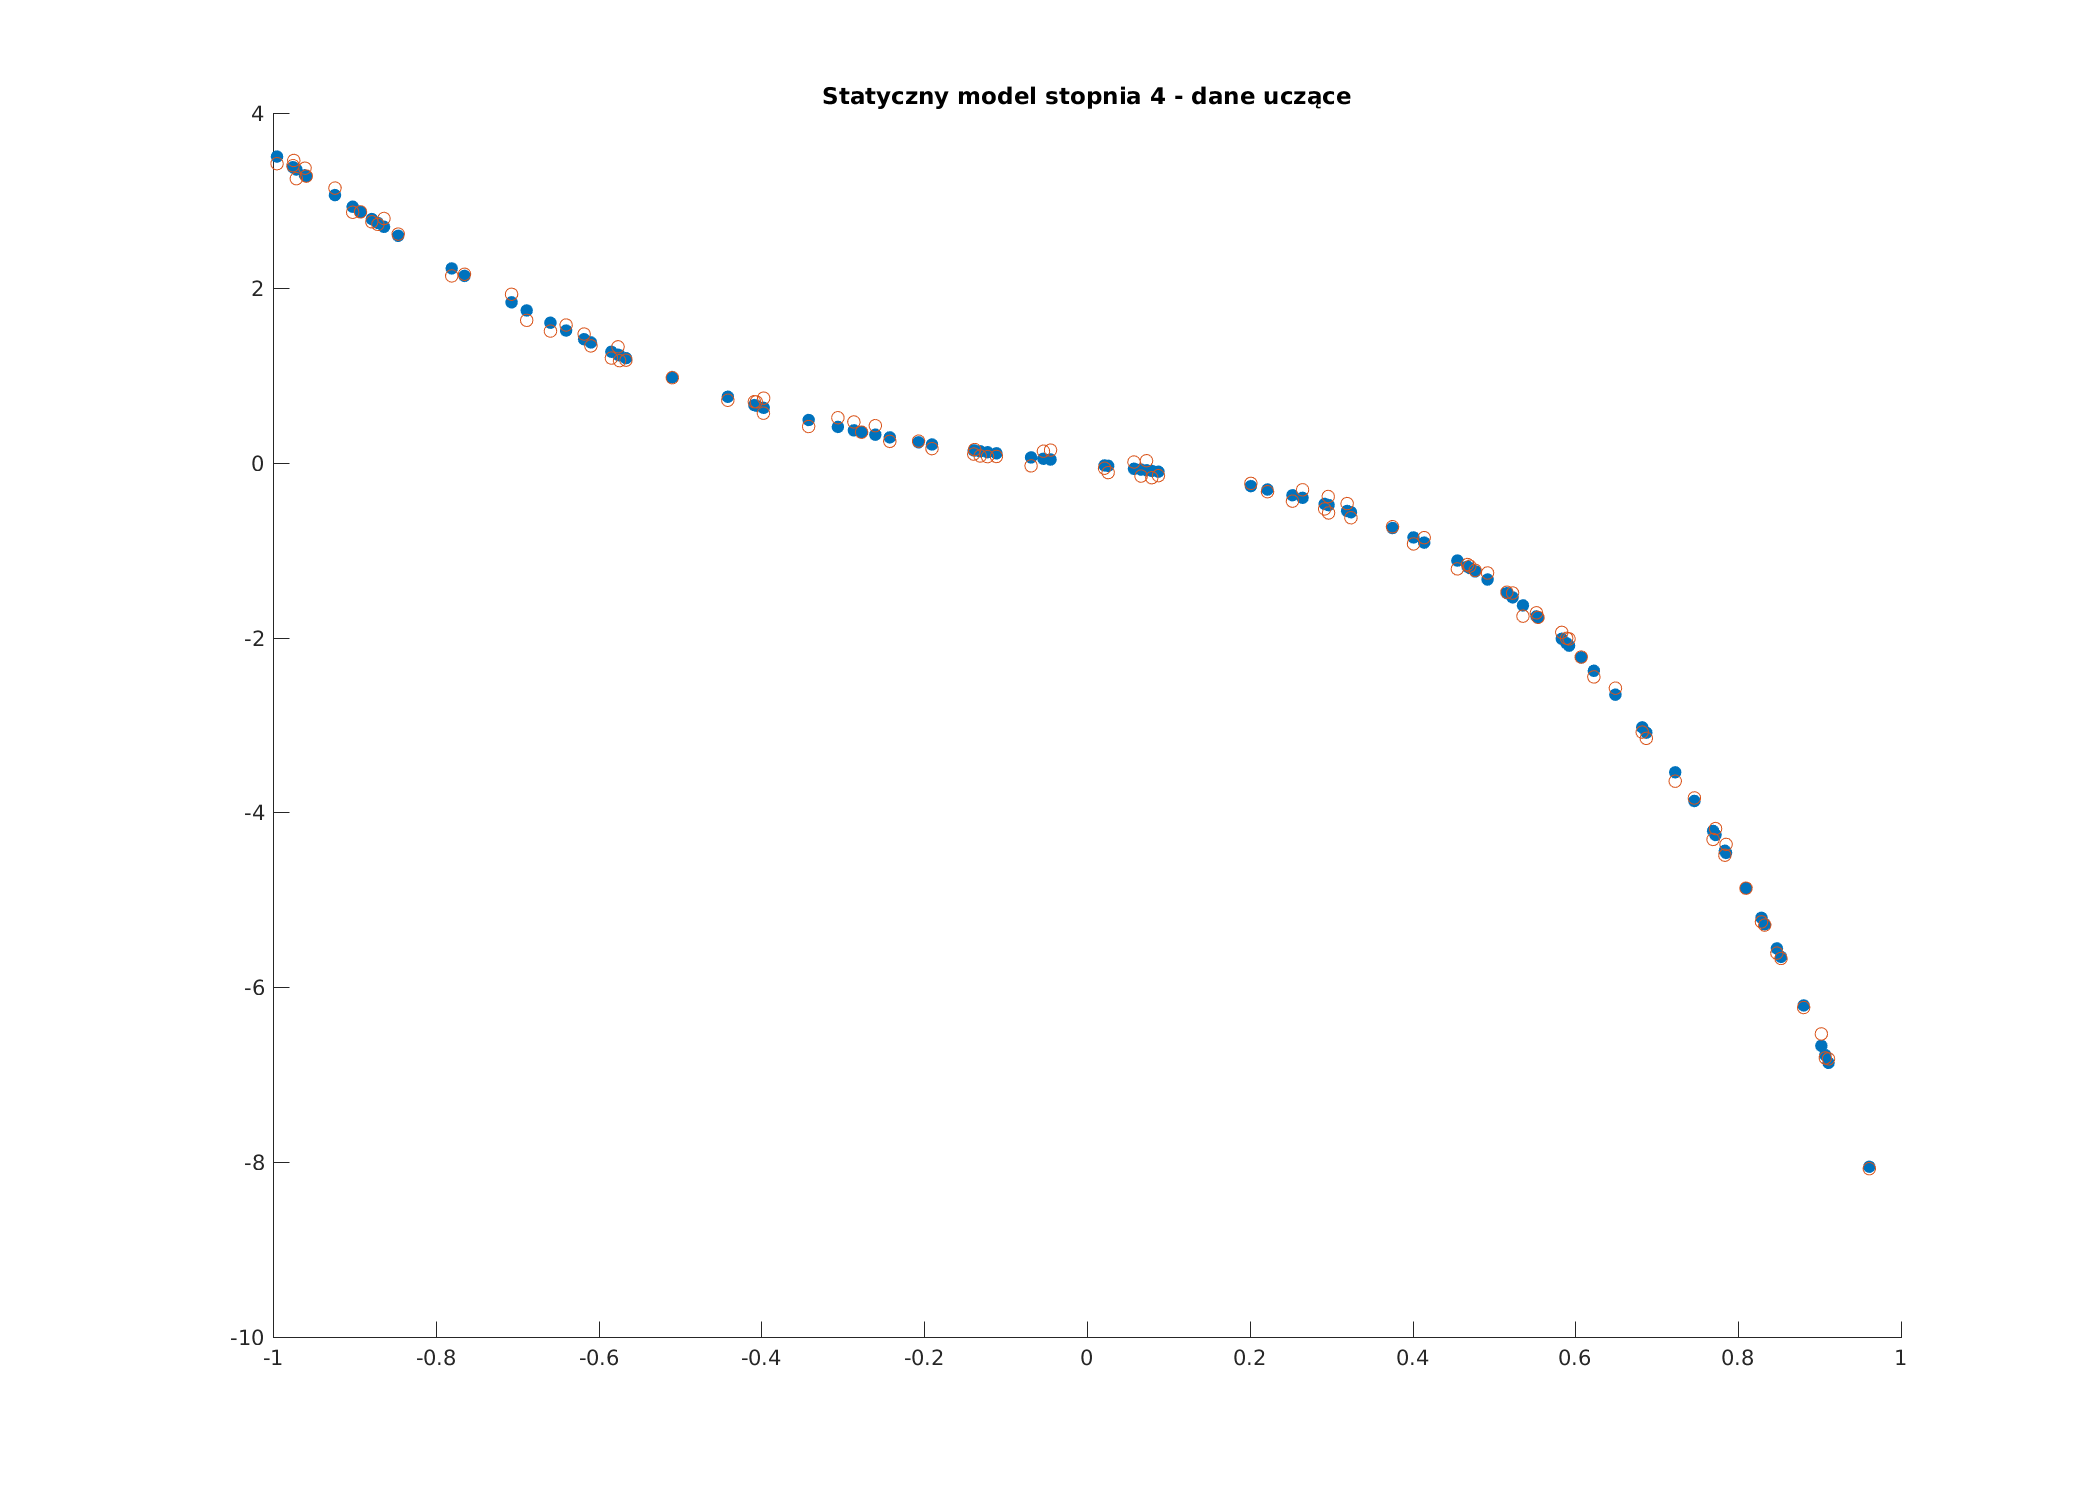
\includegraphics[scale=0.50]{dane_stat_4_ucz.png}
\caption{Model stopnia czwartego dane uczące}
\label{}
\end{figure}
\begin{figure}[H]
\centering
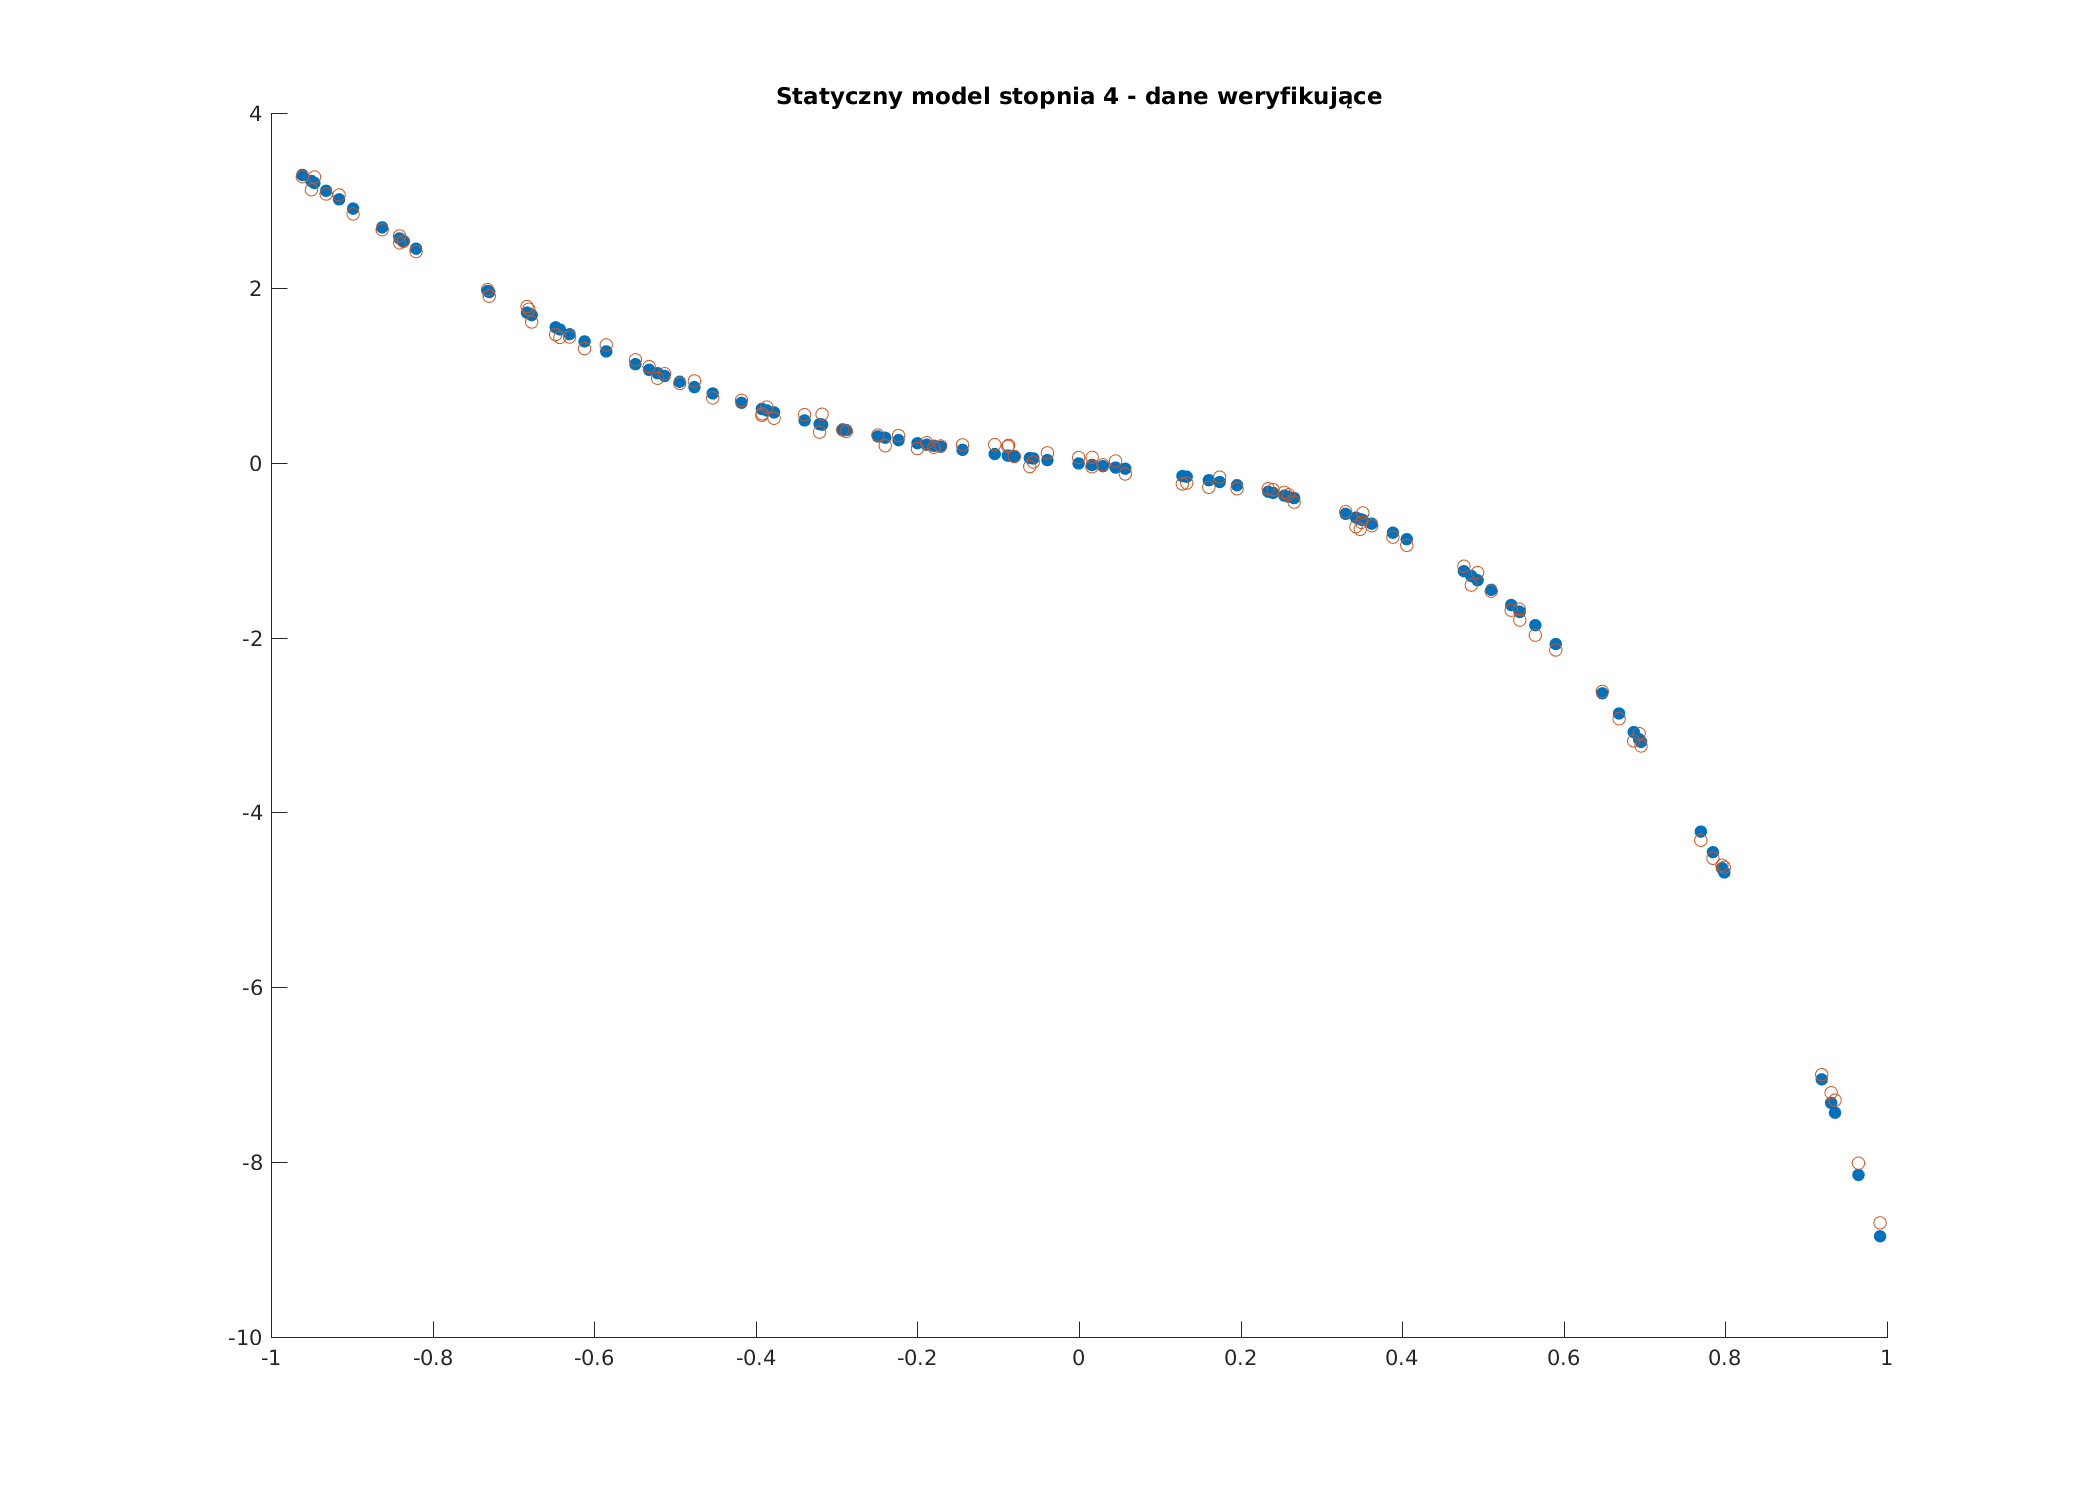
\includegraphics[scale=0.50]{dane_stat_4_wer.png}
\caption{Model stopnia czwartego dane weryfikujące}
\label{}
\end{figure}

\subsubsection{Model stopnia piątego}
\begin{figure}[H]
\centering
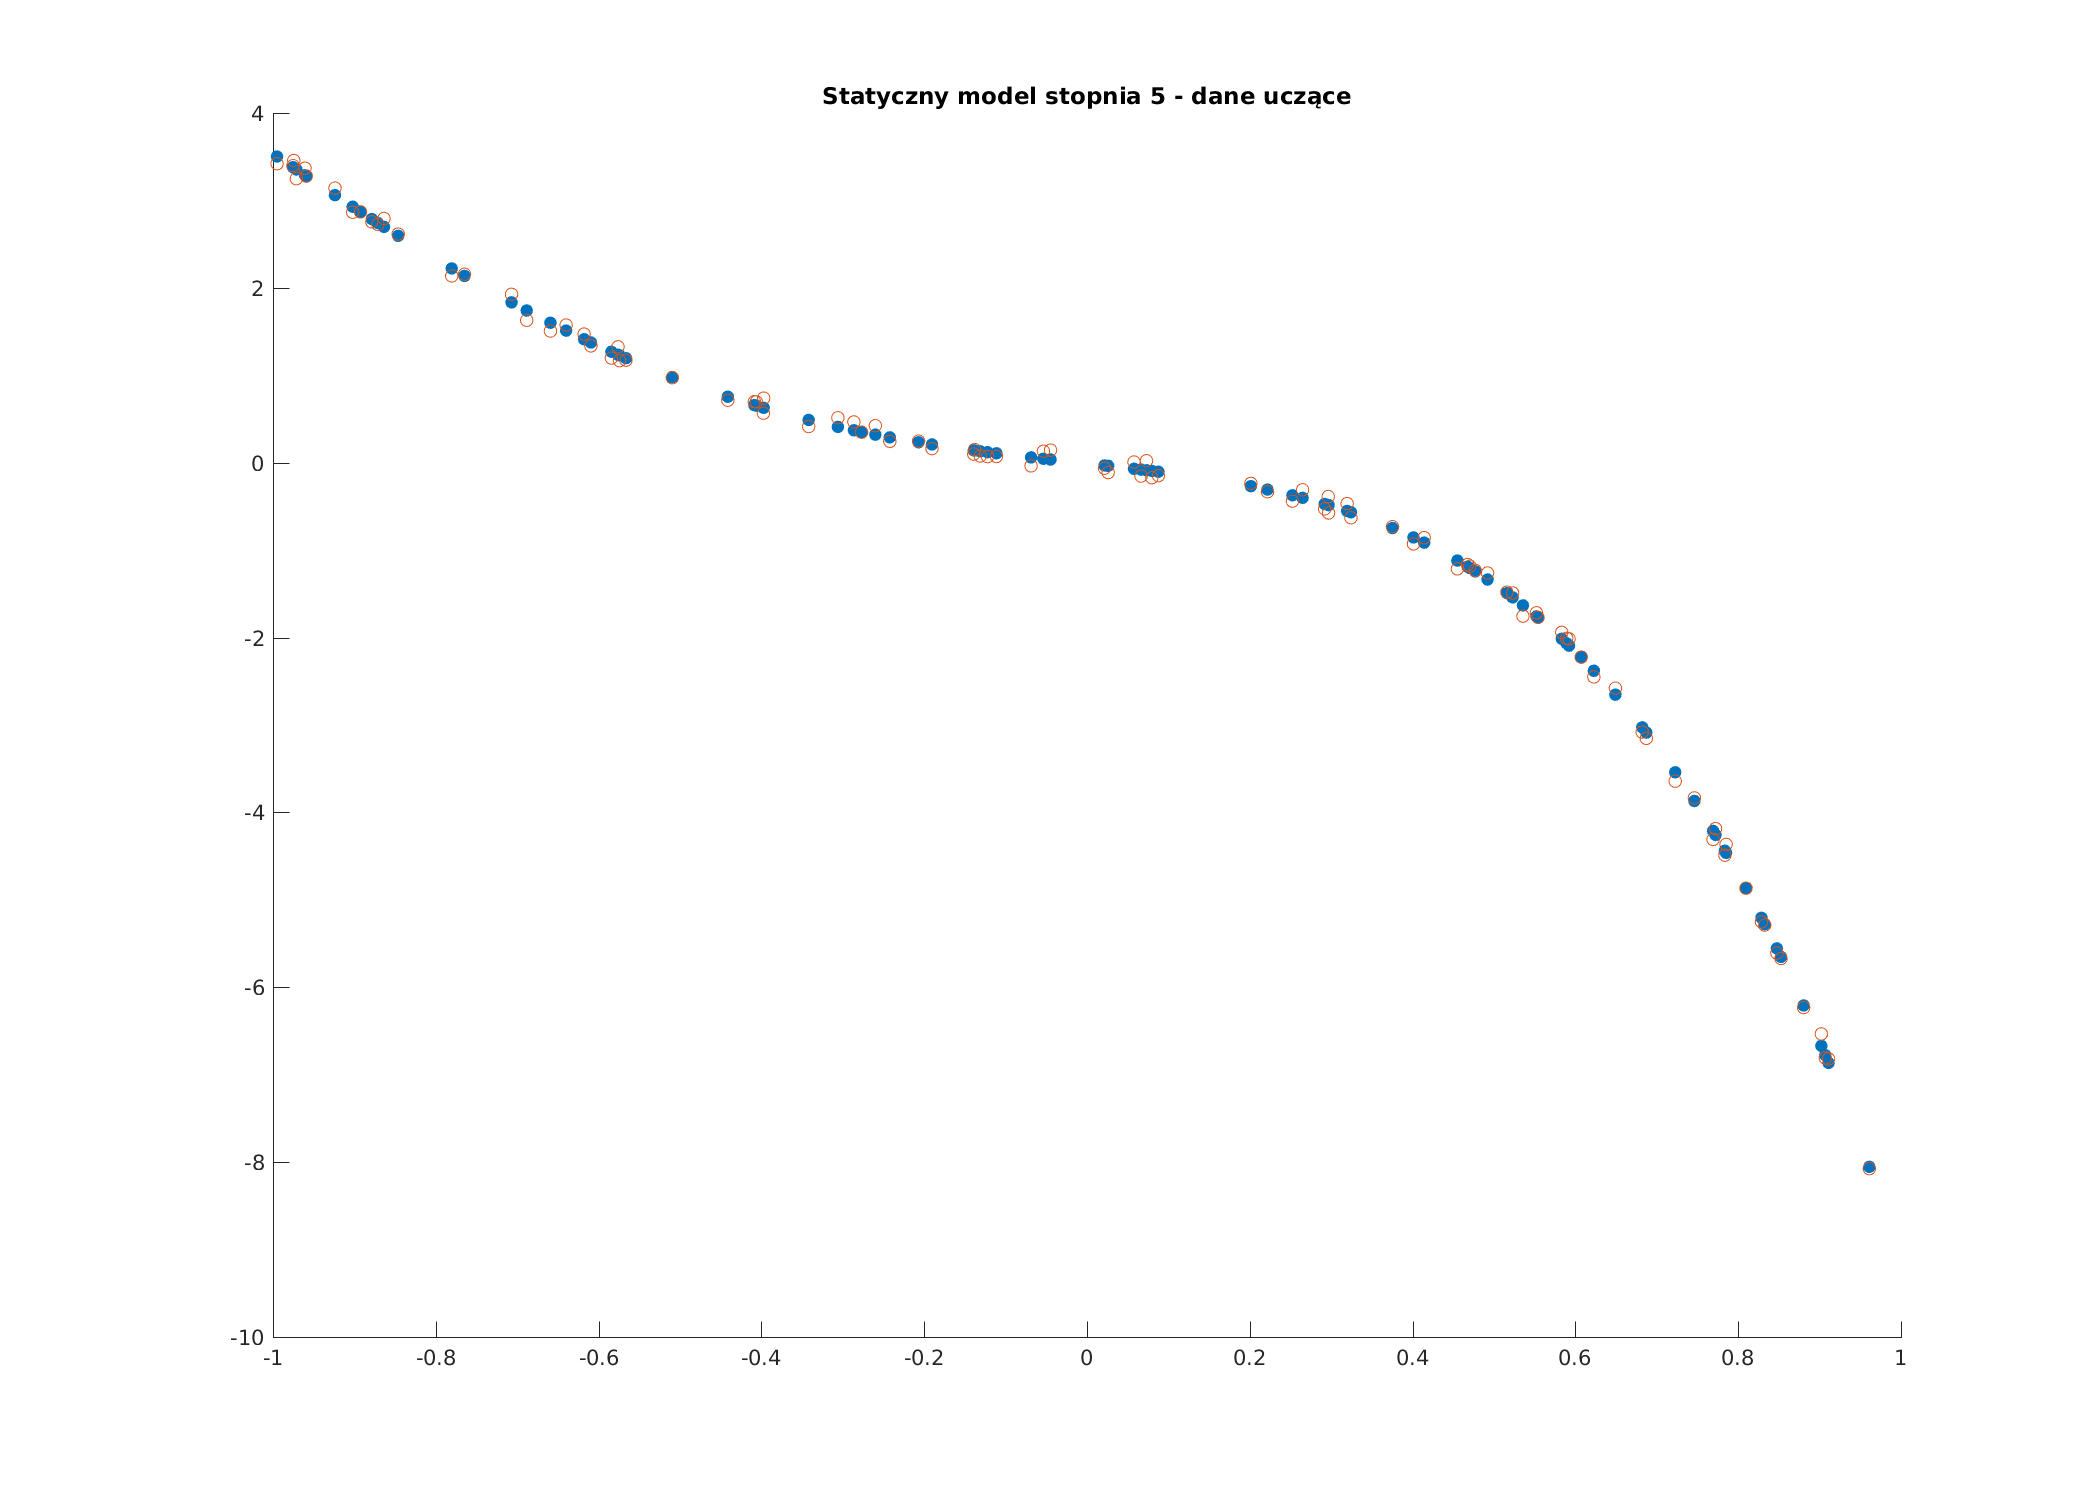
\includegraphics[scale=0.50]{dane_stat_5_ucz.png}
\caption{Model stopnia piątego dane uczące}
\label{}
\end{figure}
\begin{figure}[H]
\centering
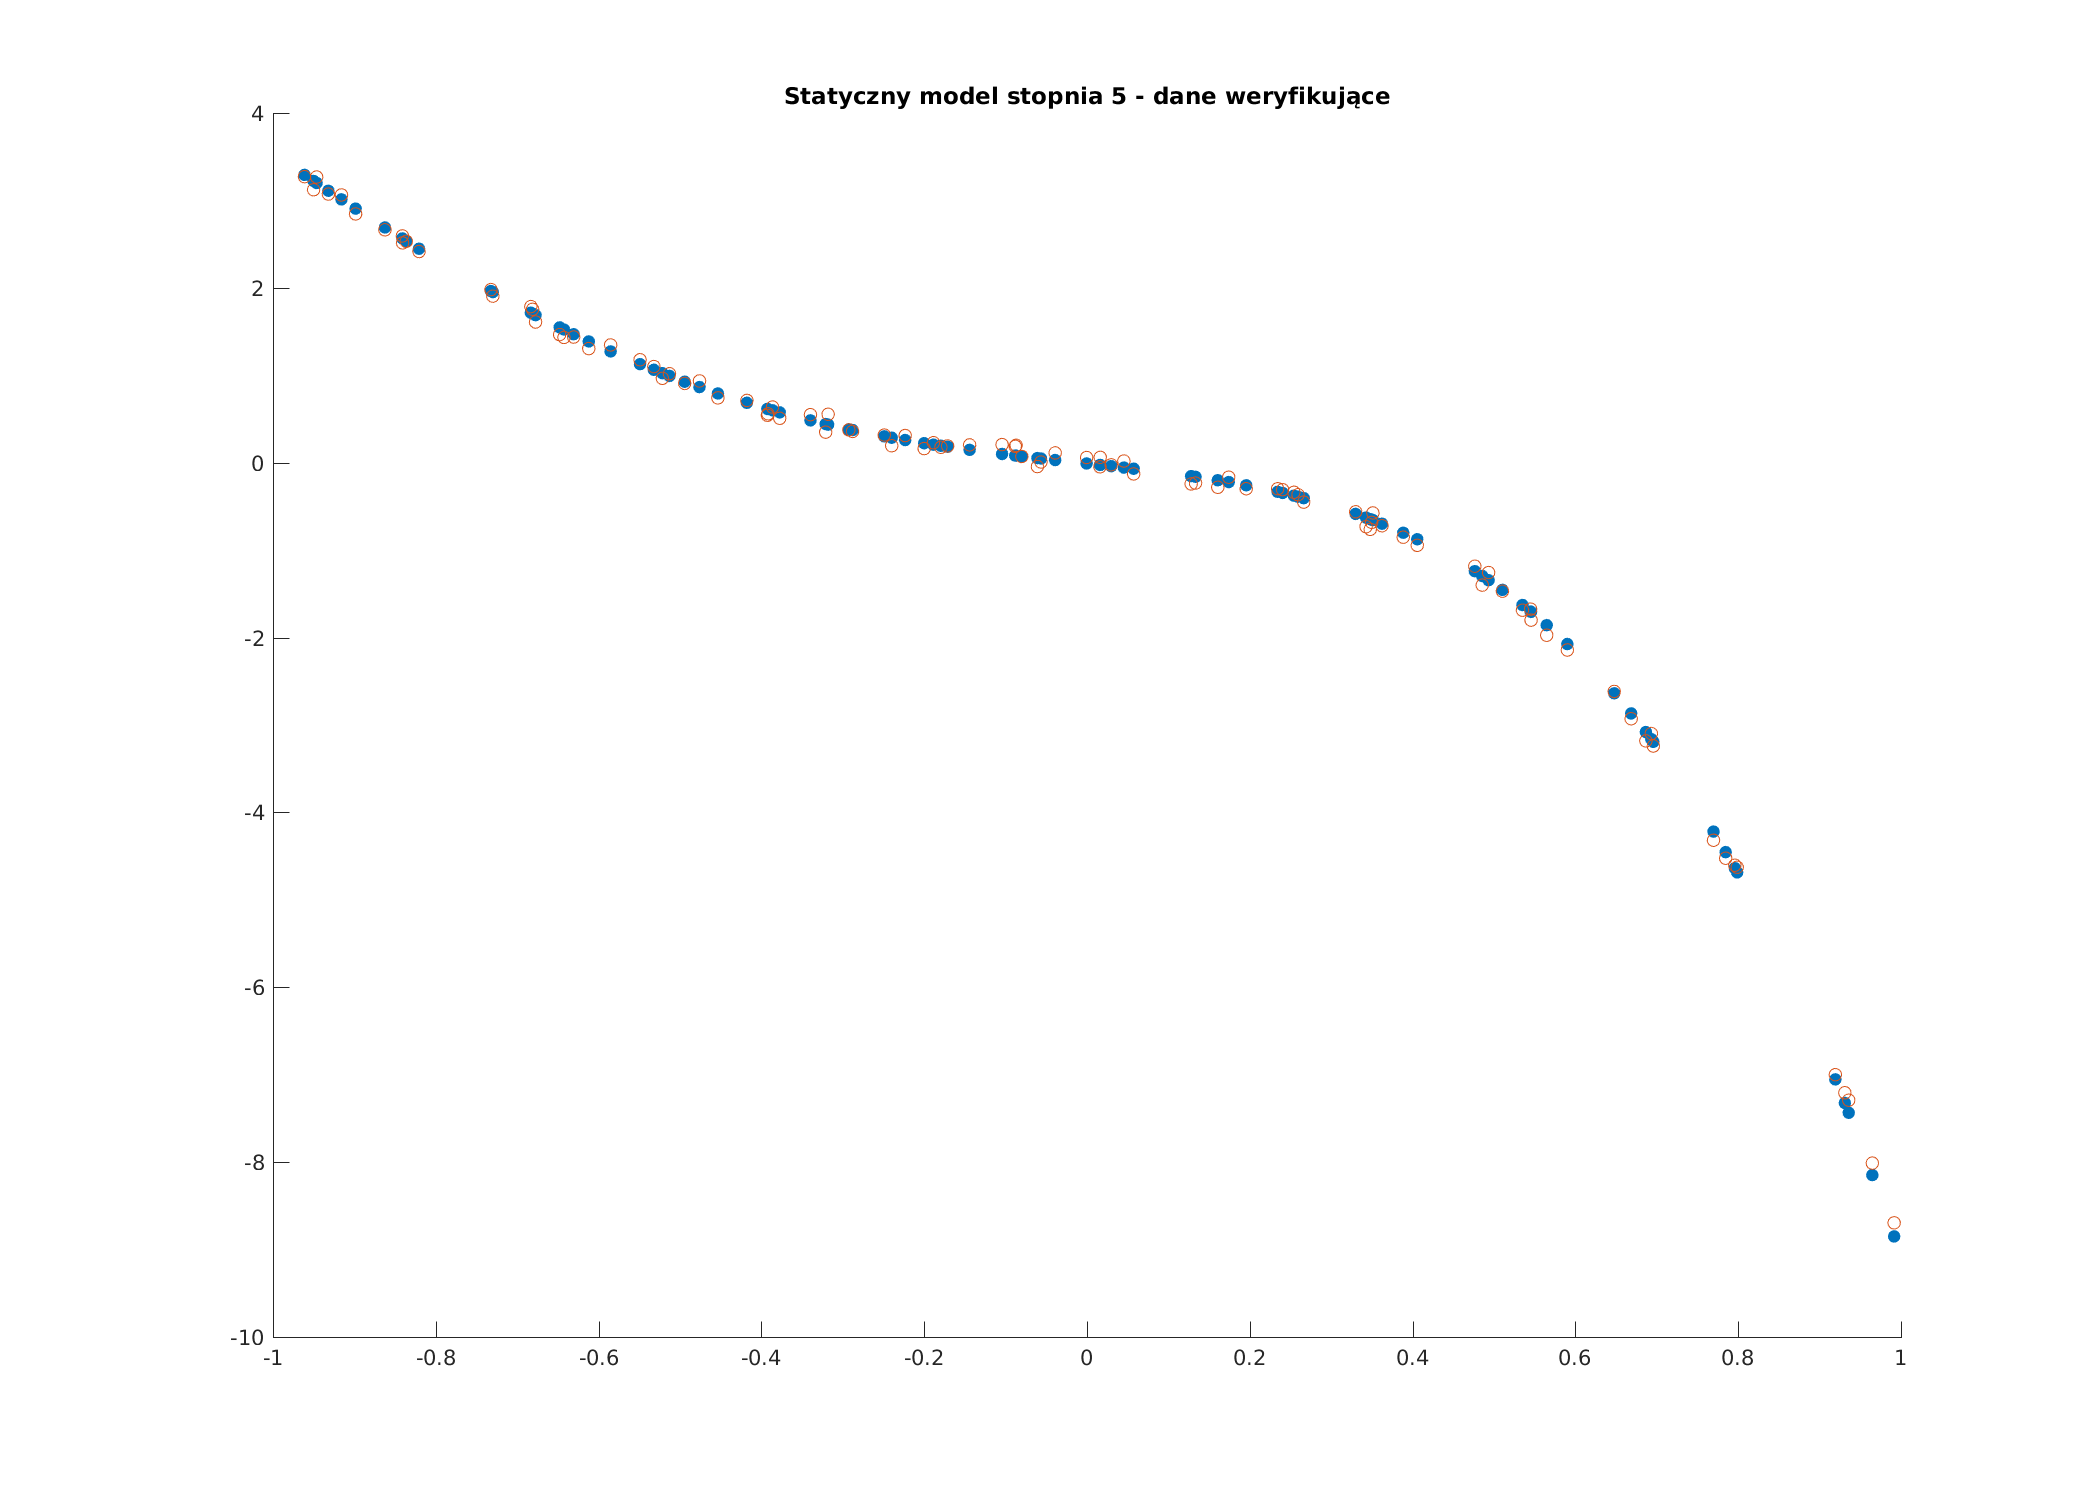
\includegraphics[scale=0.50]{dane_stat_5_wer.png}
\caption{Model stopnia piątego dane weryfikujące}
\label{}
\end{figure}


\subsubsection{Porównanie modeli nieliniowych}
Jako kryterium porównawcze stosujemy błąd dla danych weryfikujących. Zestawienie błędów modeli dla poszczególnych stopni wielomianu przedstawia tabelka: 
\begin{figure}[H]
\centering
\begin{tabular}{|c|c|c|}
\hline
	N & Dane uczące & Dane weryfikujące\\
\hline
	1 & 94.32614 & 102.8\\
\hline
	2 & 61.86064 & 65.37031\\
\hline
	3 & 3.878911 & 3.414302\\
\hline
	4 & 0.4441852 & 0.4692886\\
\hline
	5 & 0.4703329 & 0.4703329\\
\hline
\end{tabular}
\caption{Zestawienie błędów modeli}
\end{figure}
%dane_ucz_1 9.432614e+01 
%dane_wer_1 1.028000e+02 
%dane_ucz_2 6.186064e+01 
%ane_wer_2 6.537031e+01 
%dane_ucz_3 3.878911e+00 
%ane_wer_3 3.414302e+00 
%dane_ucz_4 4.441852e-01 
%dane_wer_4 4.692886e-01 
%dane_ucz_5 4.441751e-01 
%dane_wer_5 4.703329e-01 

\subsection{Wybór najlepszego modelu}
Najmniejszy błąd dla zbioru weryfikującego występuje w przypadku modelu będącego wielomianem czwartego stopnia, dla stopnia wyższego następuje pogorszenie modelu.


\section{Identyfikacja modelu dynamicznego}
W celu badania modeli dynamicznych został napisany skrypt pakietu Matlab znajdujący się w pliku \textbf{dynamiczne.m}. 
Odpowiada on za poprawne wczytanie danych modelu oraz identyfikację modelu, obliczanie błędów, oraz rysowanie wykresów. 

\subsection{Reprezentacja graficzna danych dynamicznych}
\subsubsection{Zbiór uczący}
\begin{figure}[H]
\centering
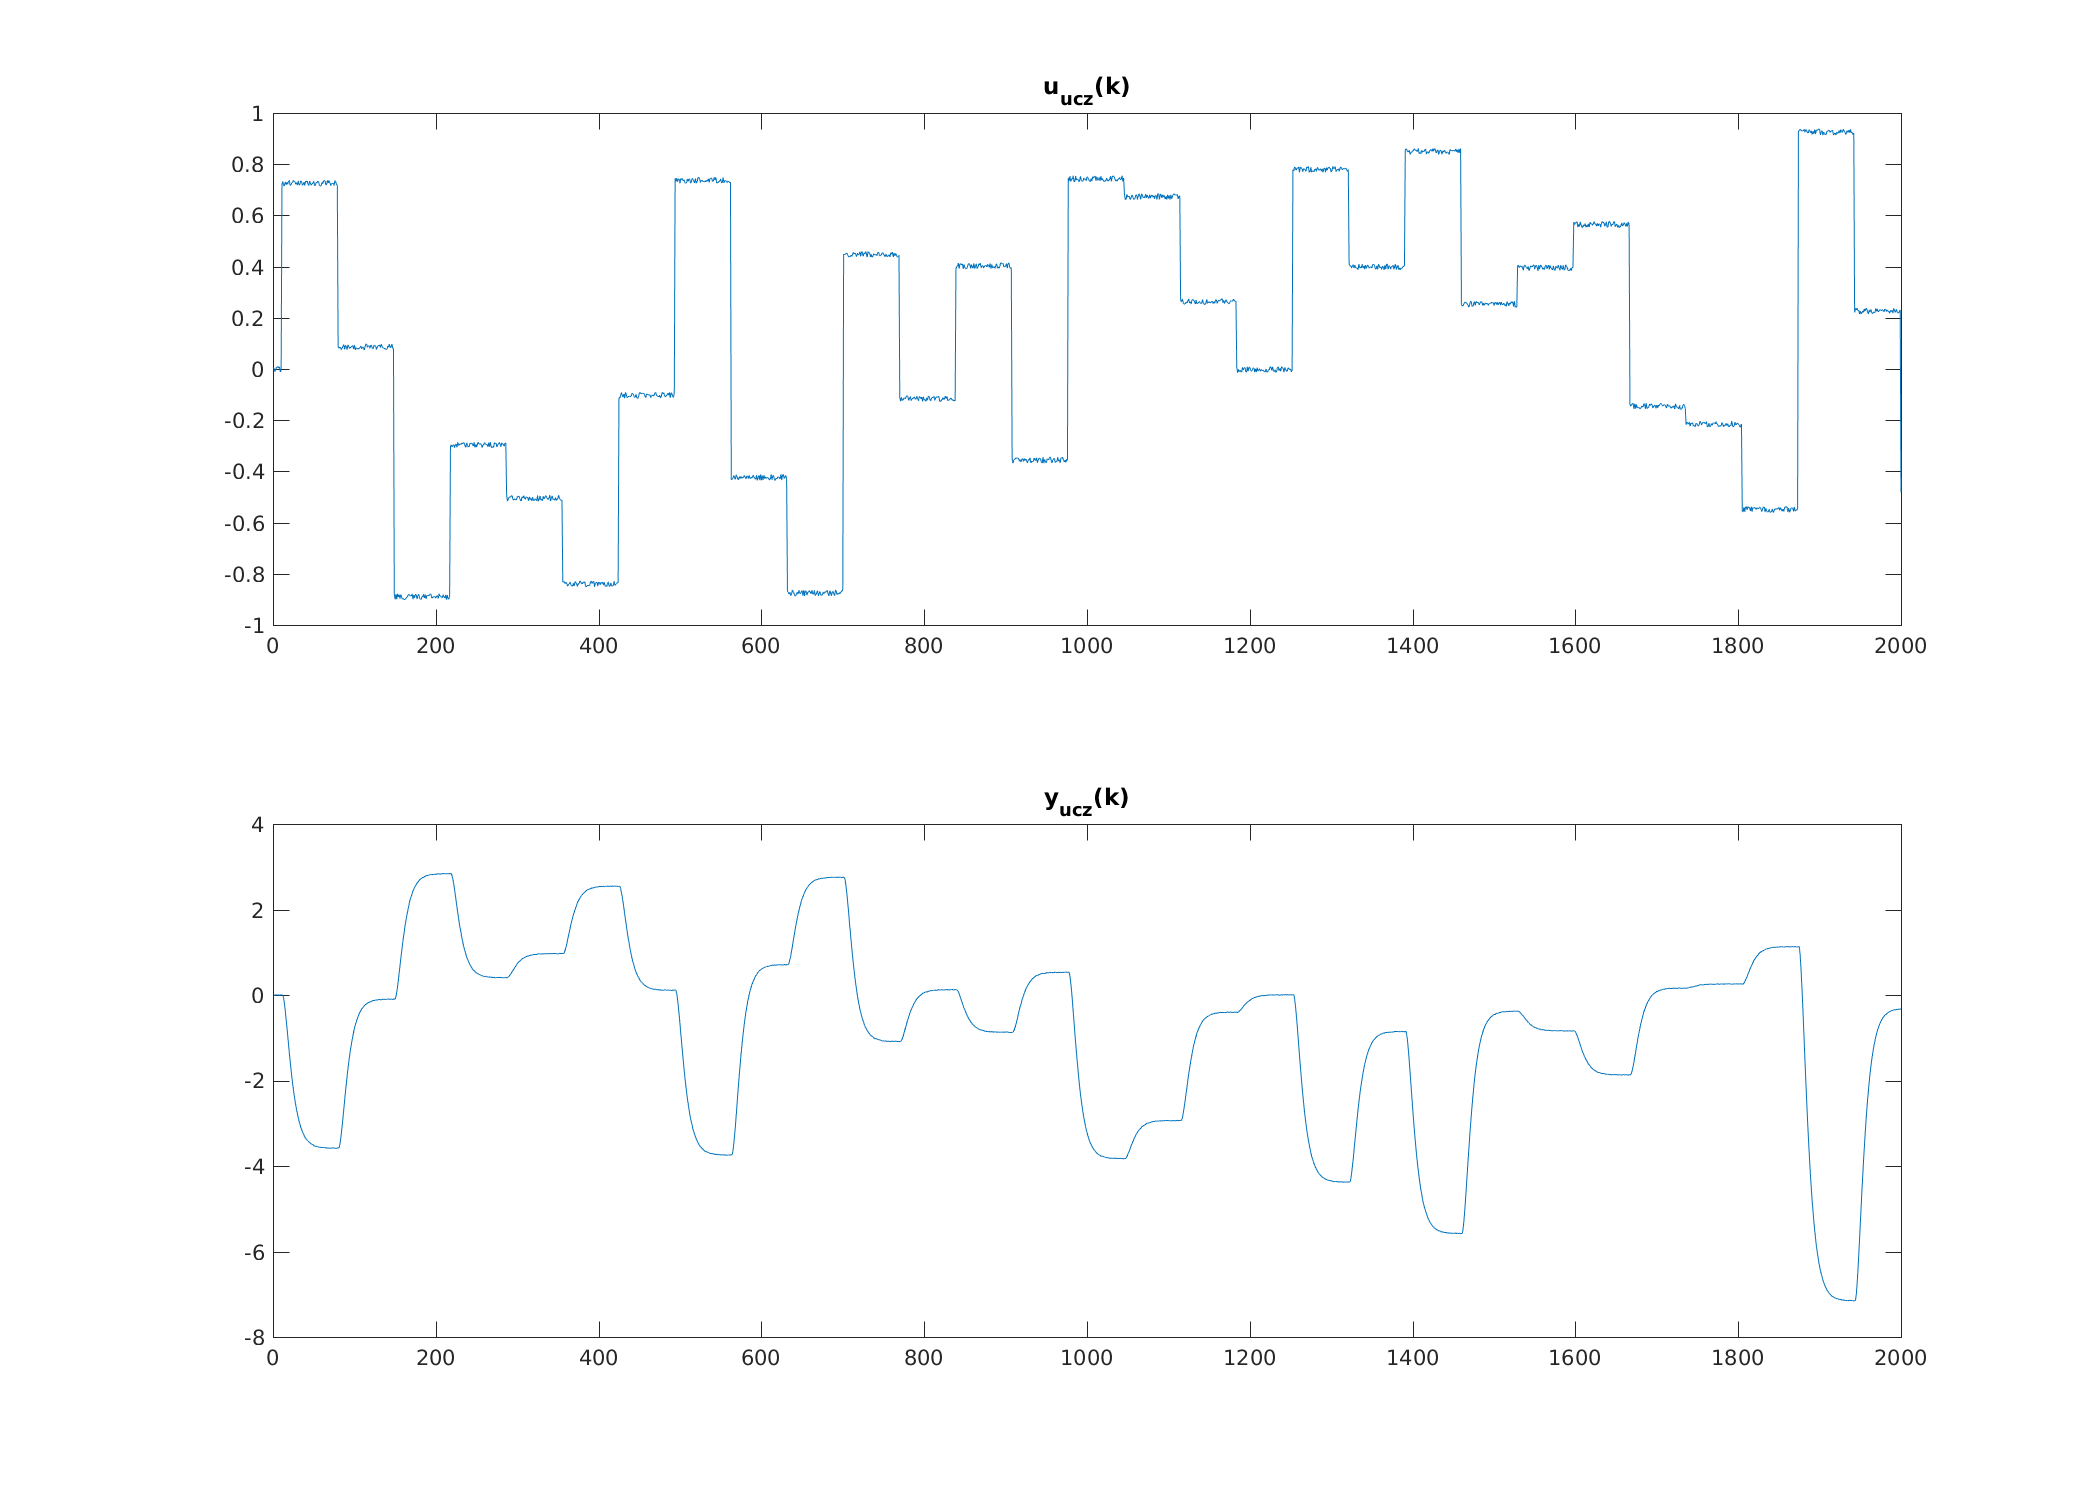
\includegraphics[scale=0.50]{dane_dyn_ucz.png}
\caption{Reprezentacja graficzna zbioru uczącego }
\label{}
\end{figure}

\subsubsection{Zbiór weryfikujący}
\begin{figure}[H]
\centering
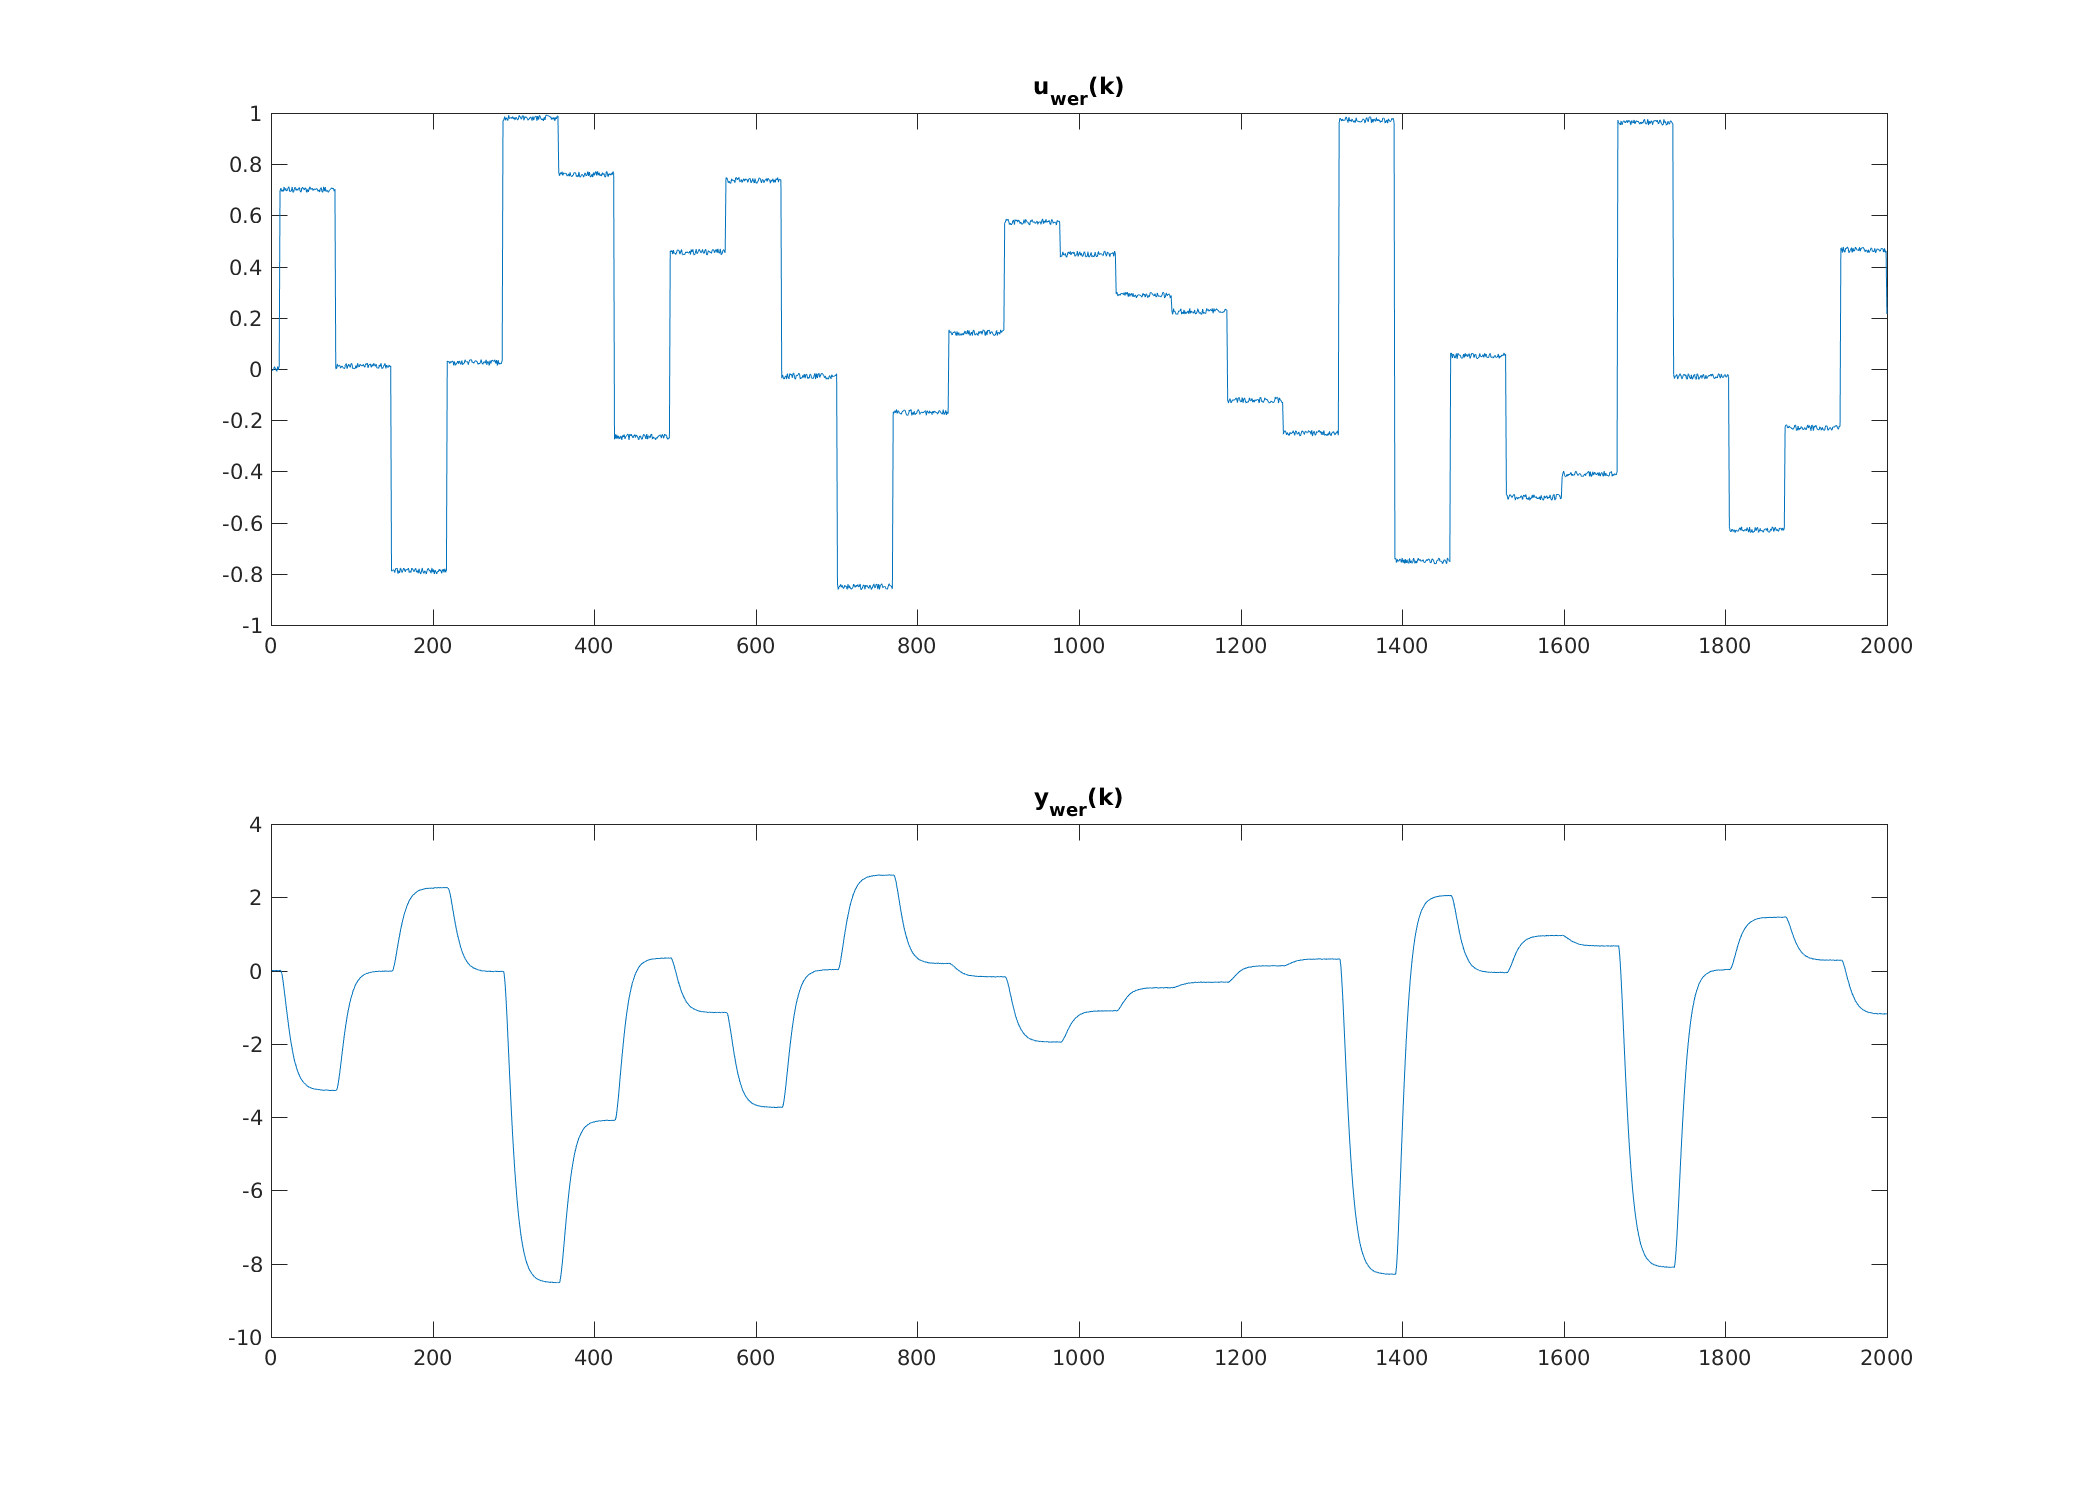
\includegraphics[scale=0.50]{dane_dyn_wer.png}
\caption{Reprezentacja graficzna zbioru weryfikującego}
\label{}
\end{figure}

\subsection{Dynamiczne modele liniowe}
Na tym etapie badać będziemy model przybliżony wielomianami pierwszego stopnia o różnych rzędach dynamiki, w trybie z rekurencją i bez rekurencji. 

\subsubsection{Rzędu pierwszego}
Dla pierwszego rzędu dynamiki wielomian pierwszego stopnia ma postać : 
$$y(k) = b_1u(k-1) + a_1y(k-1)$$
\begin{figure}[H]
\centering
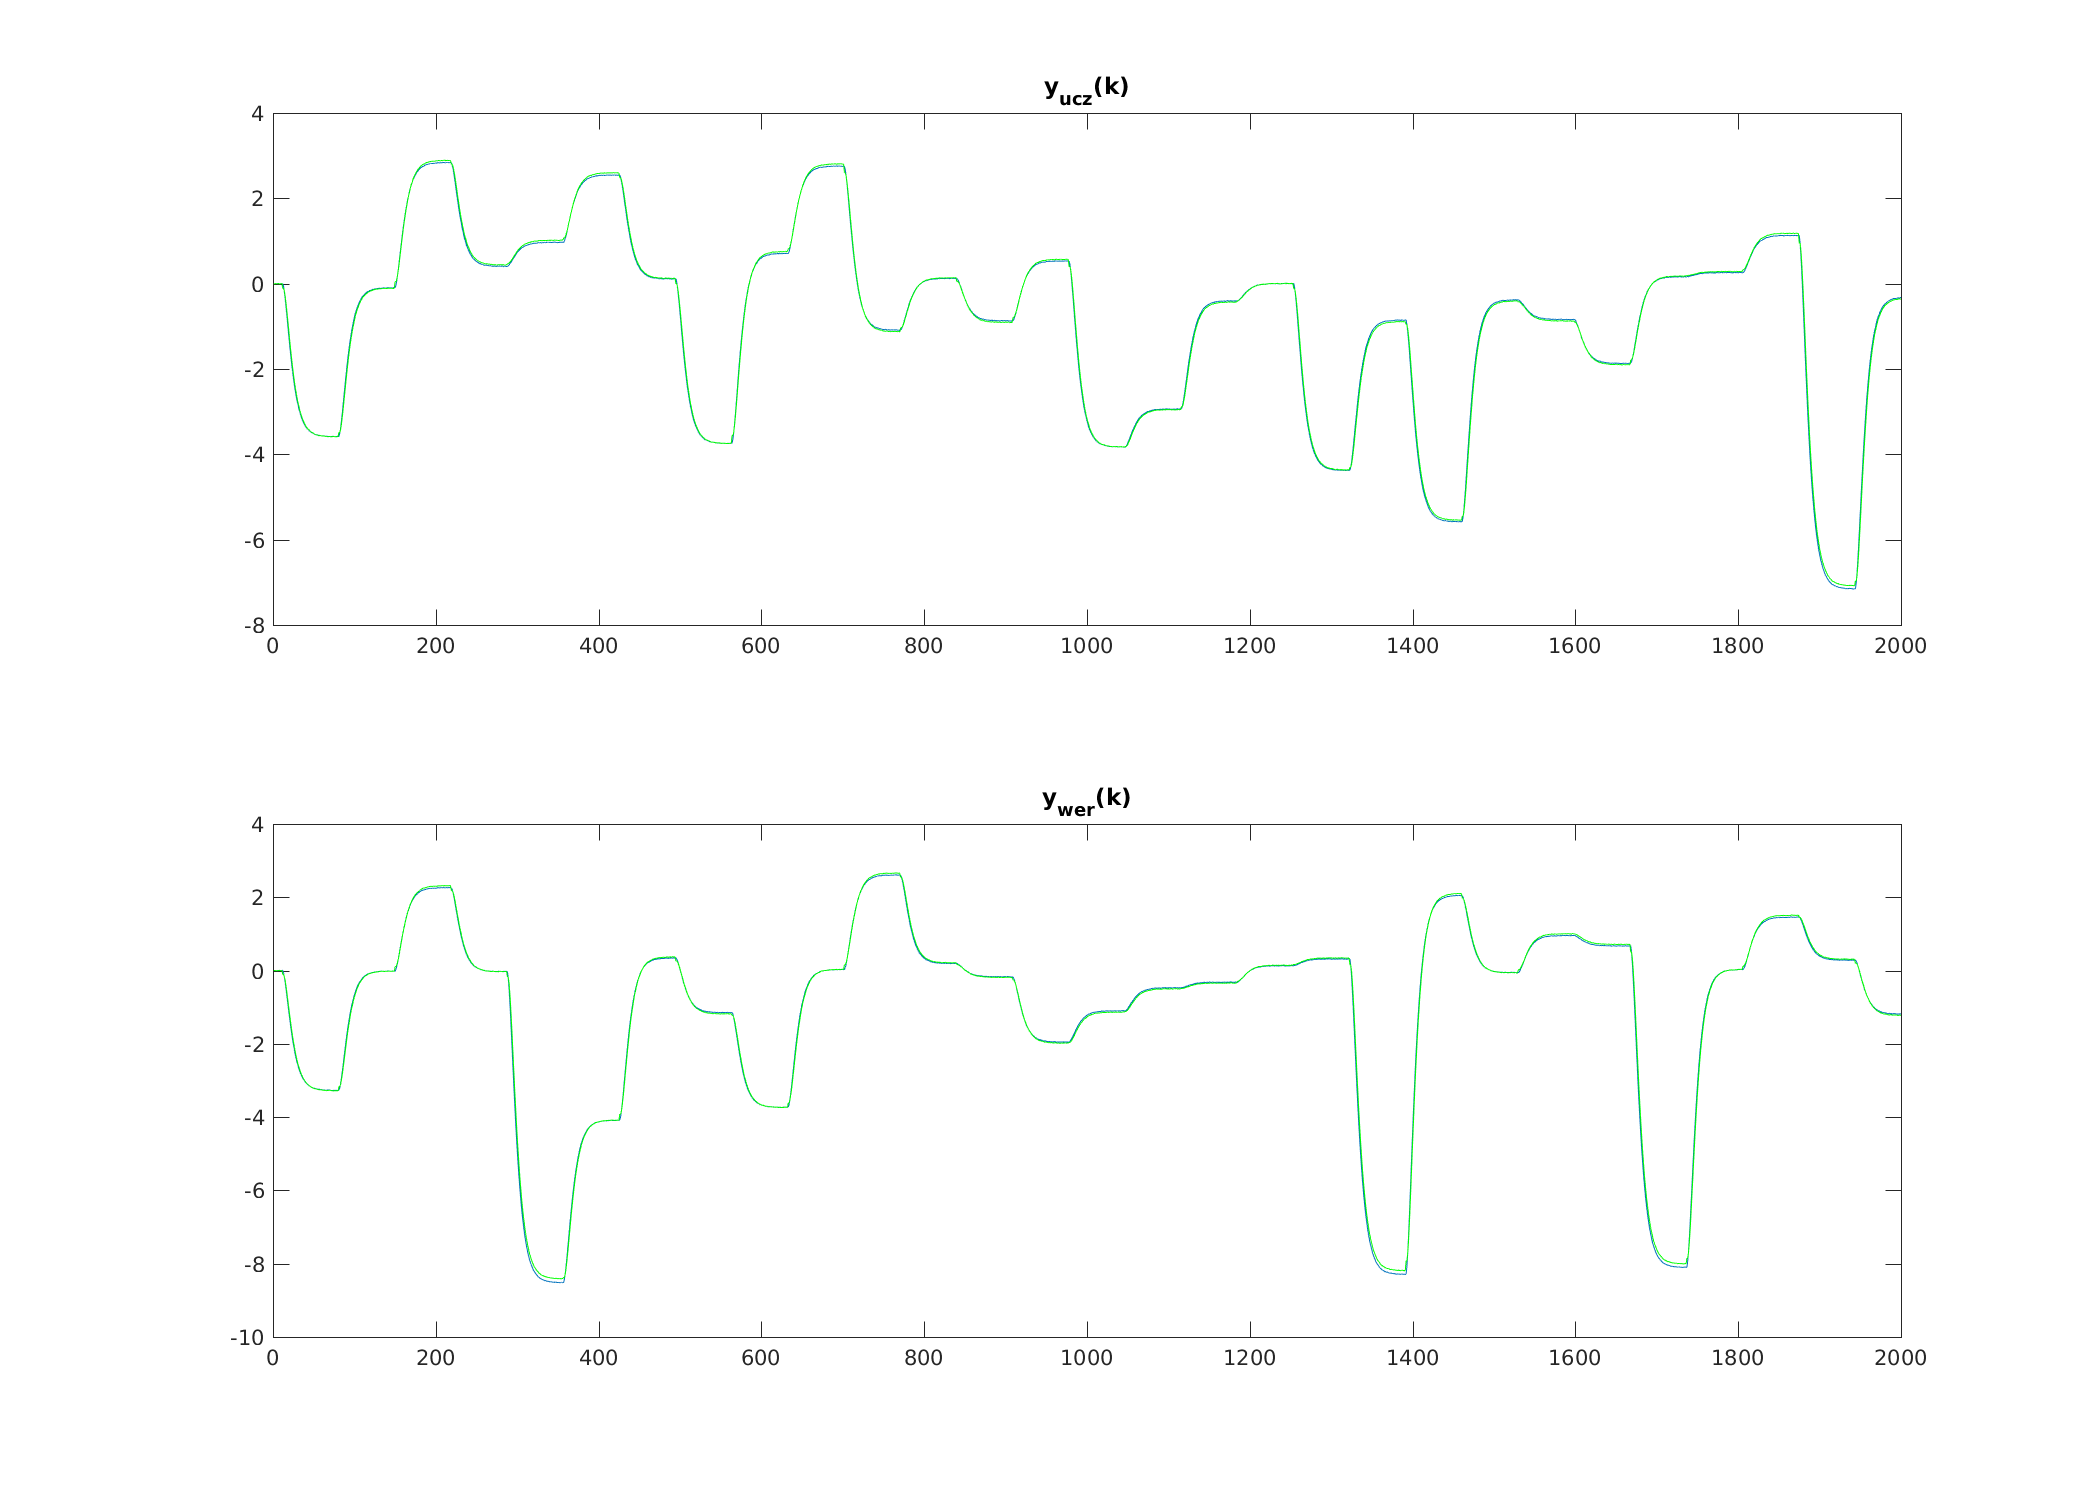
\includegraphics[scale=0.50]{dane_dyn_mod_brek_D_1.png}
\caption{Model z pierwszym rzędem dynamiki w trybie bez rekurencji }
\label{}
\end{figure}
\begin{figure}[H]
\centering
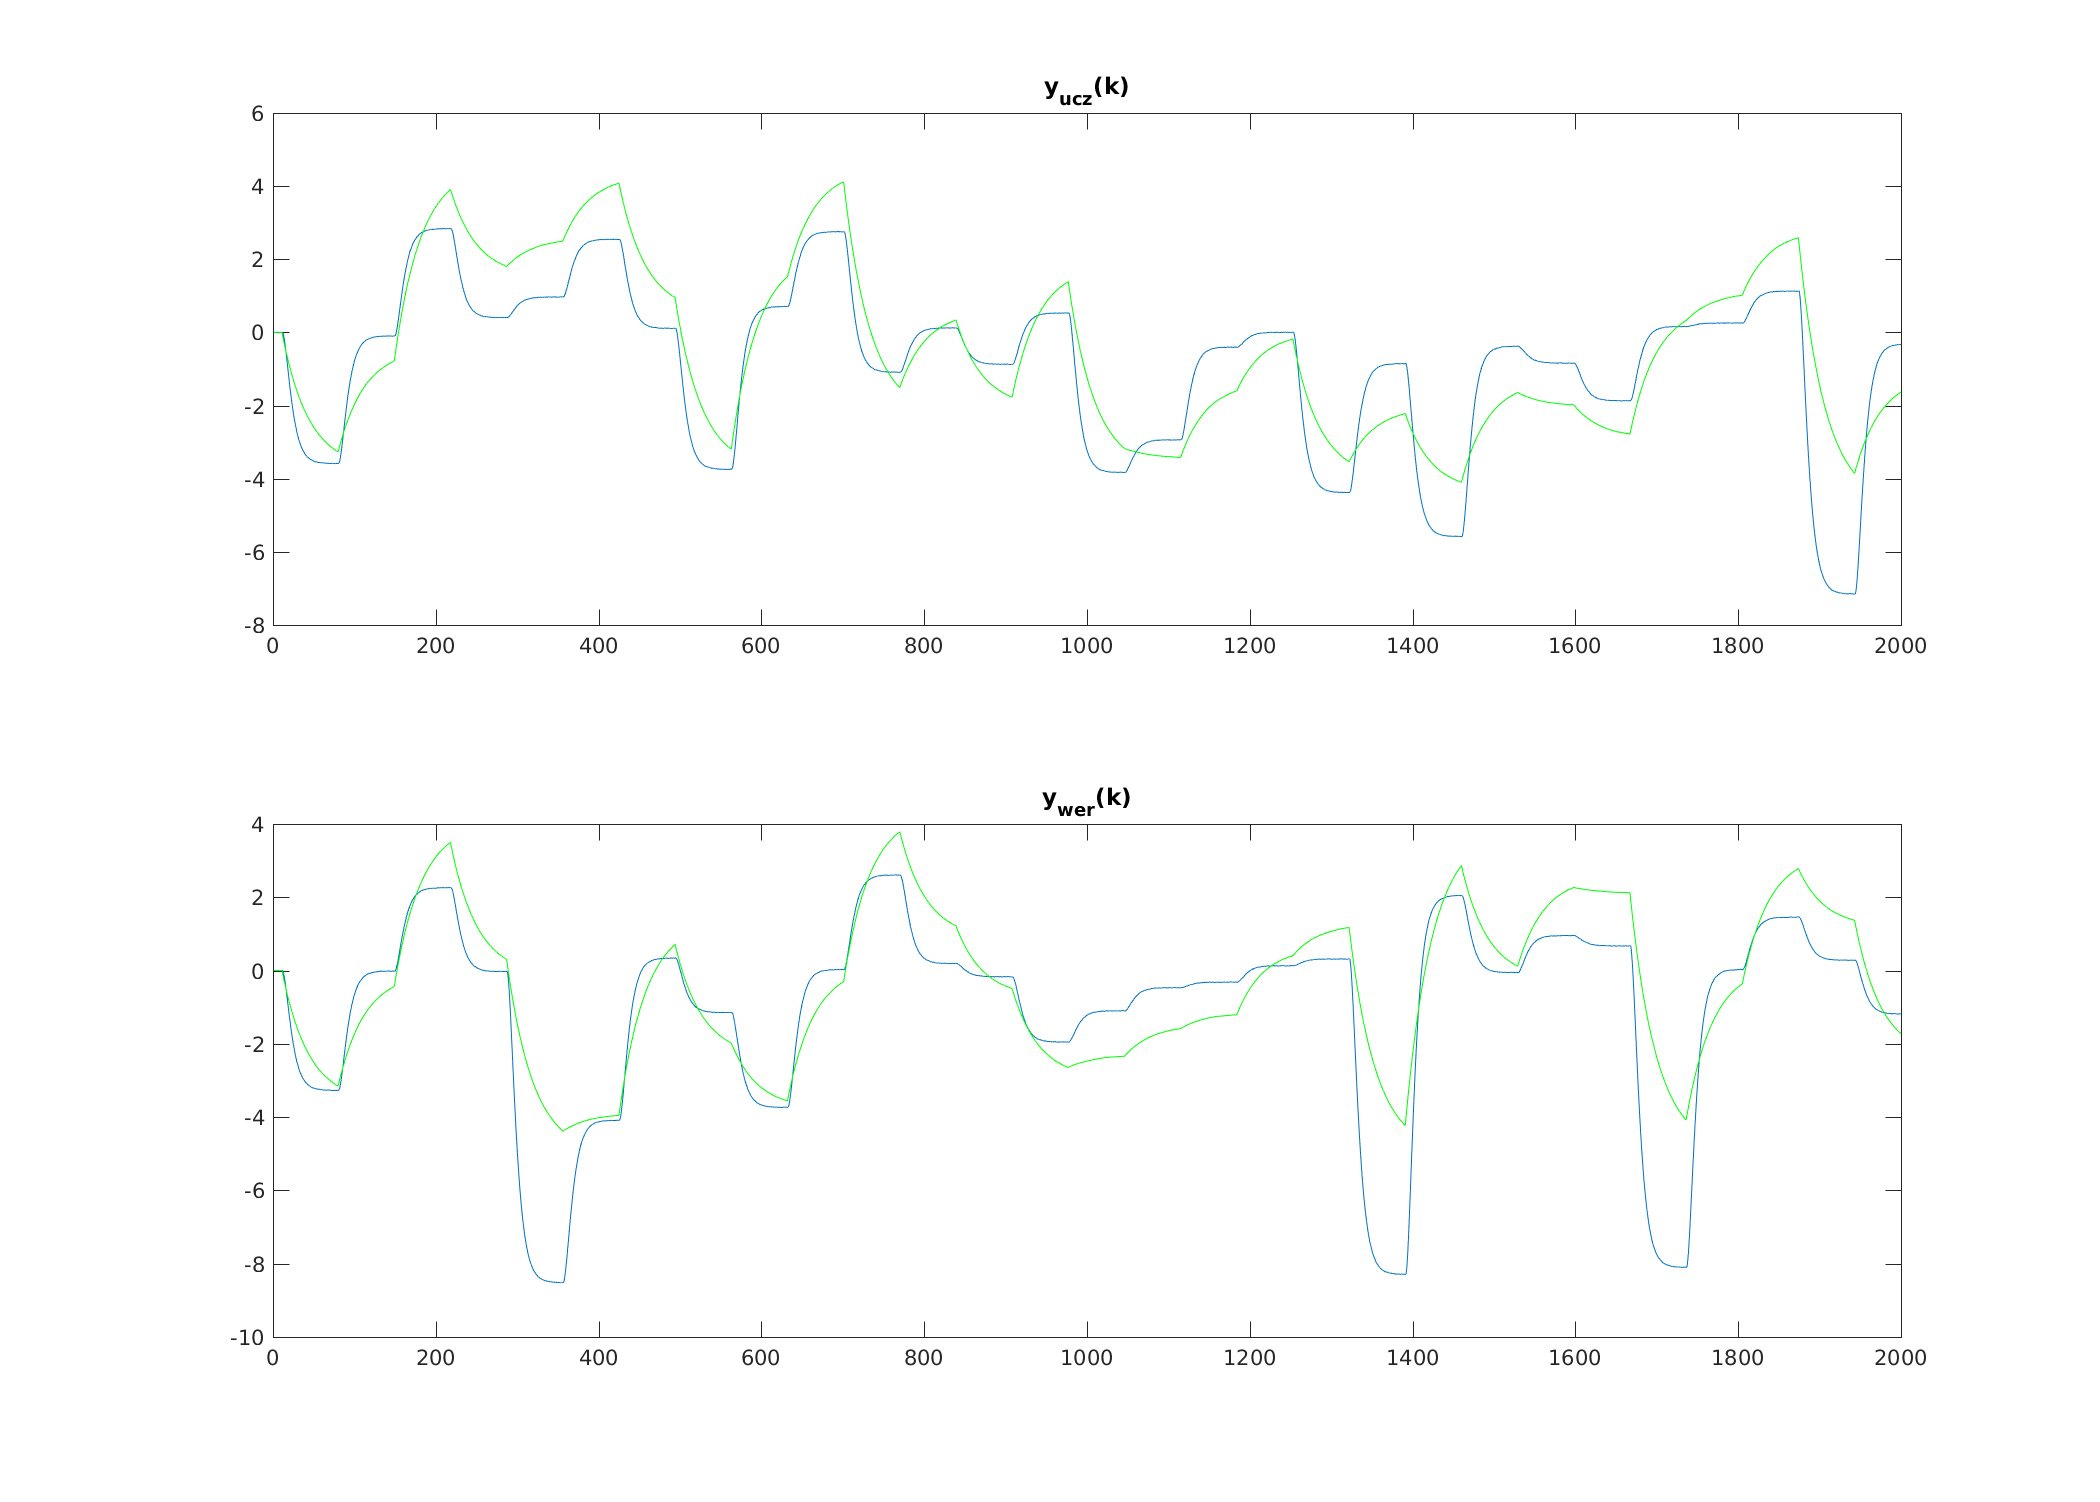
\includegraphics[scale=0.50]{dane_dyn_mod_rek_D_1.png}
\caption{Model z pierwszym rzędem dynamiki w trybie z rekurencją }
\label{}
\end{figure}


\subsubsection{Rzędu drugiego}
Dla drugiego rzędu dynamiki wielomian pierwszego stopnia ma postać : 
$$y(k) = b_1u(k-1)+b_2u(k-2) + a_1y(k-1)+a_2y(k-2)$$
\begin{figure}[H]
\centering
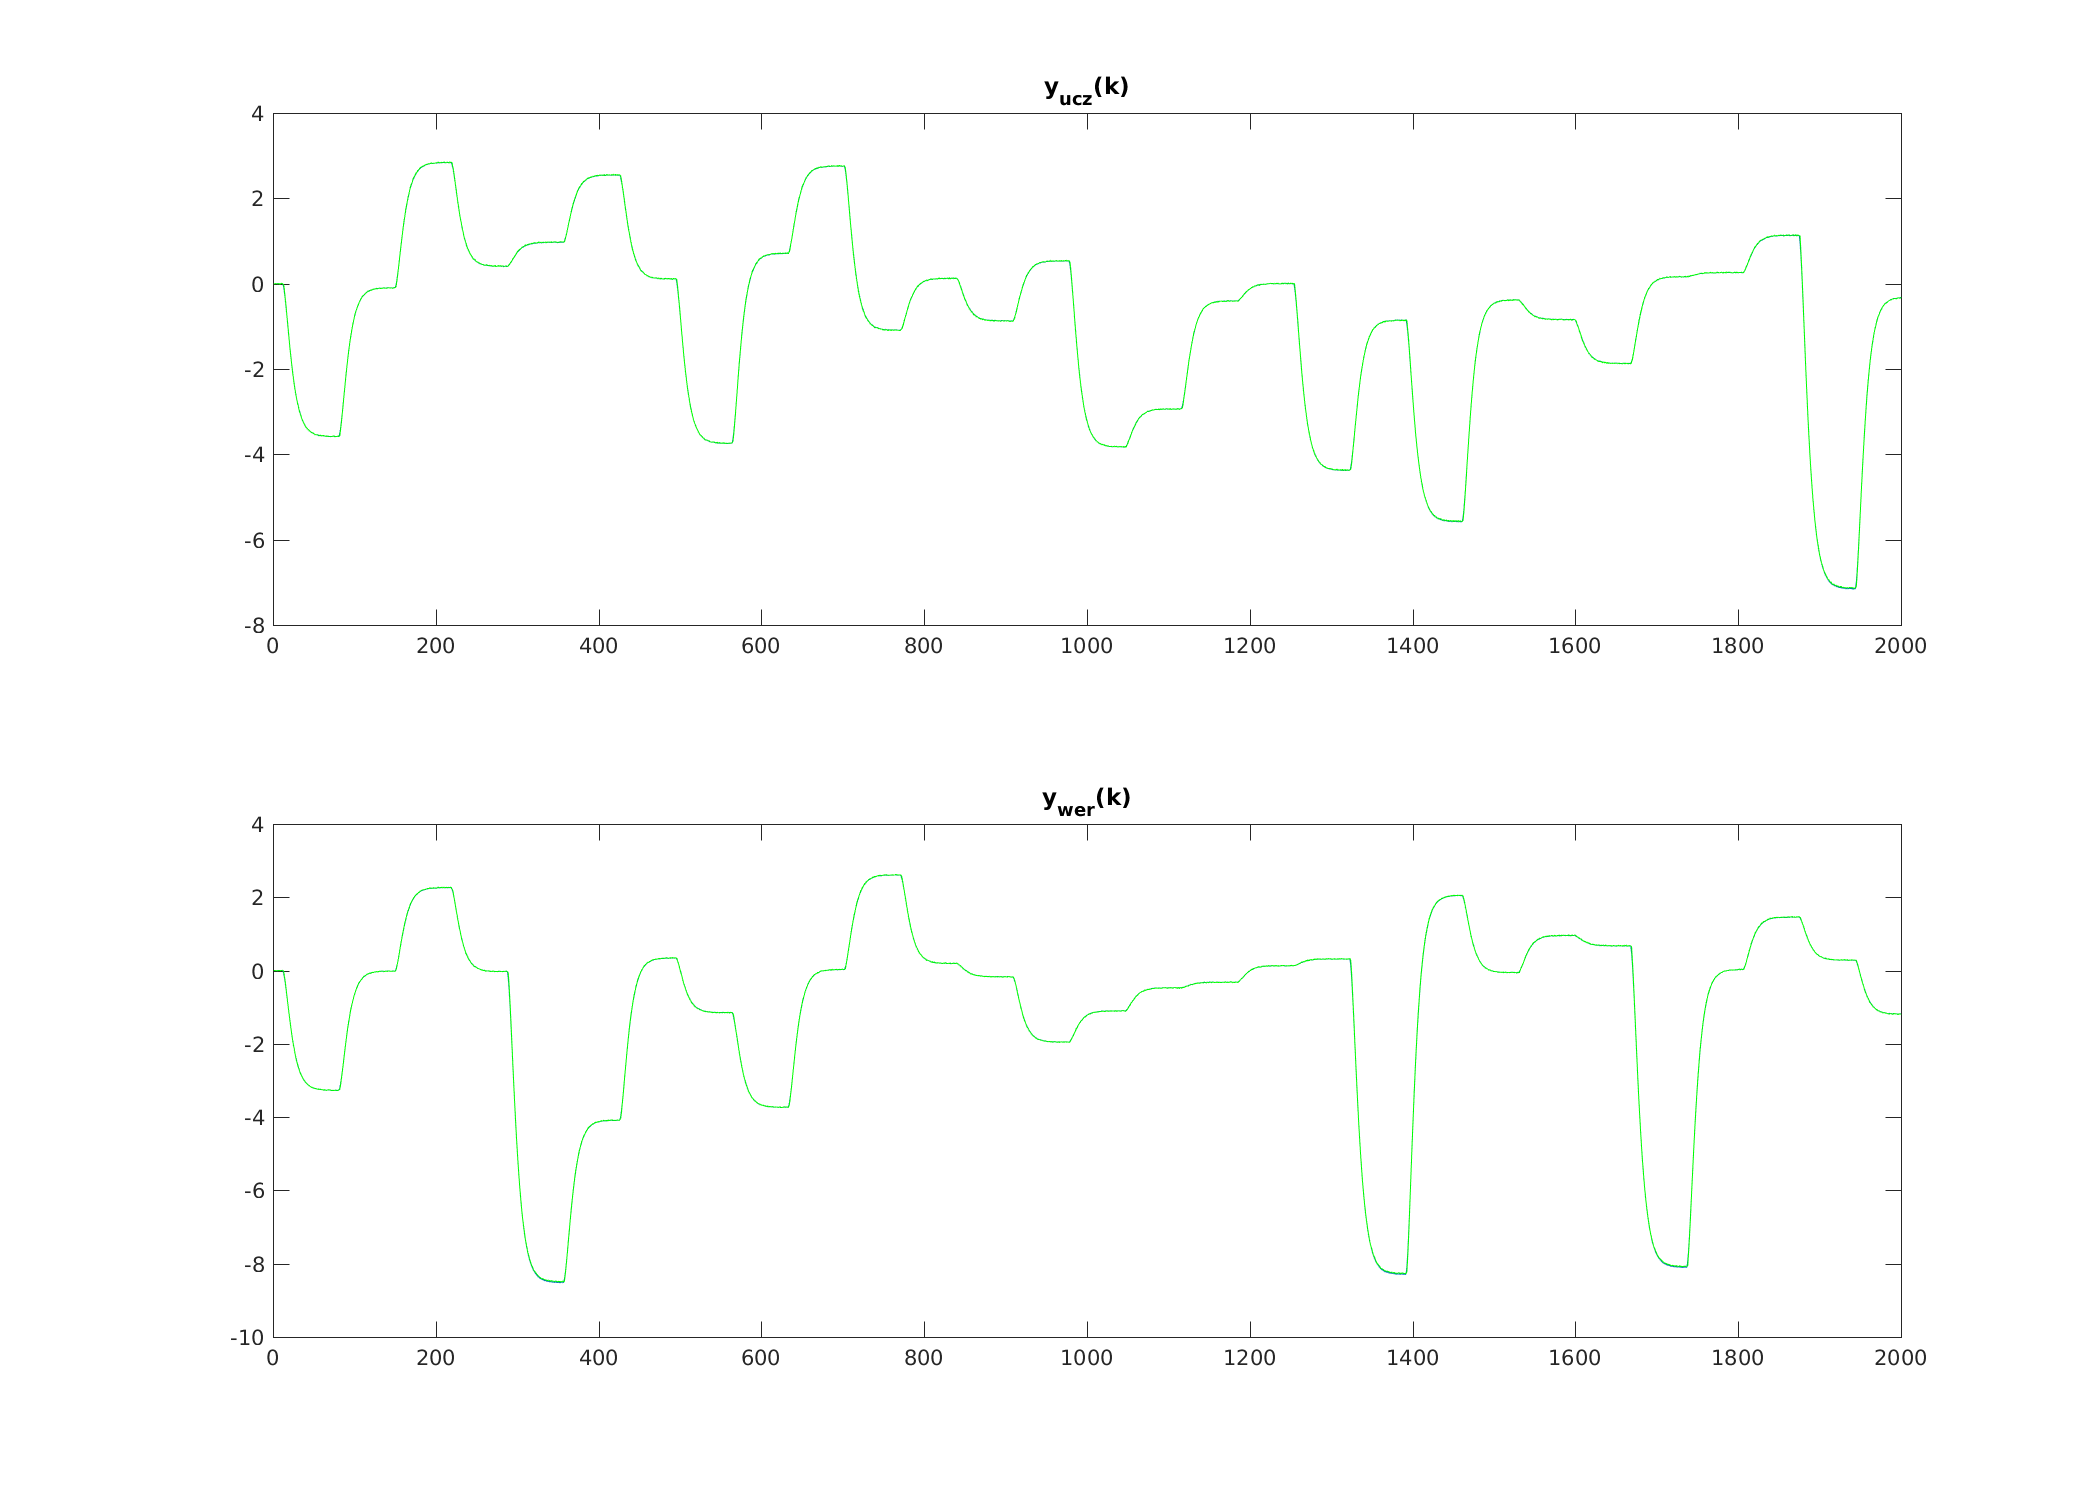
\includegraphics[scale=0.50]{dane_dyn_mod_brek_D_2.png}
\caption{Model z drugim rzędem dynamiki w trybie bez rekurencji }
\label{}
\end{figure}
\begin{figure}[H]
\centering
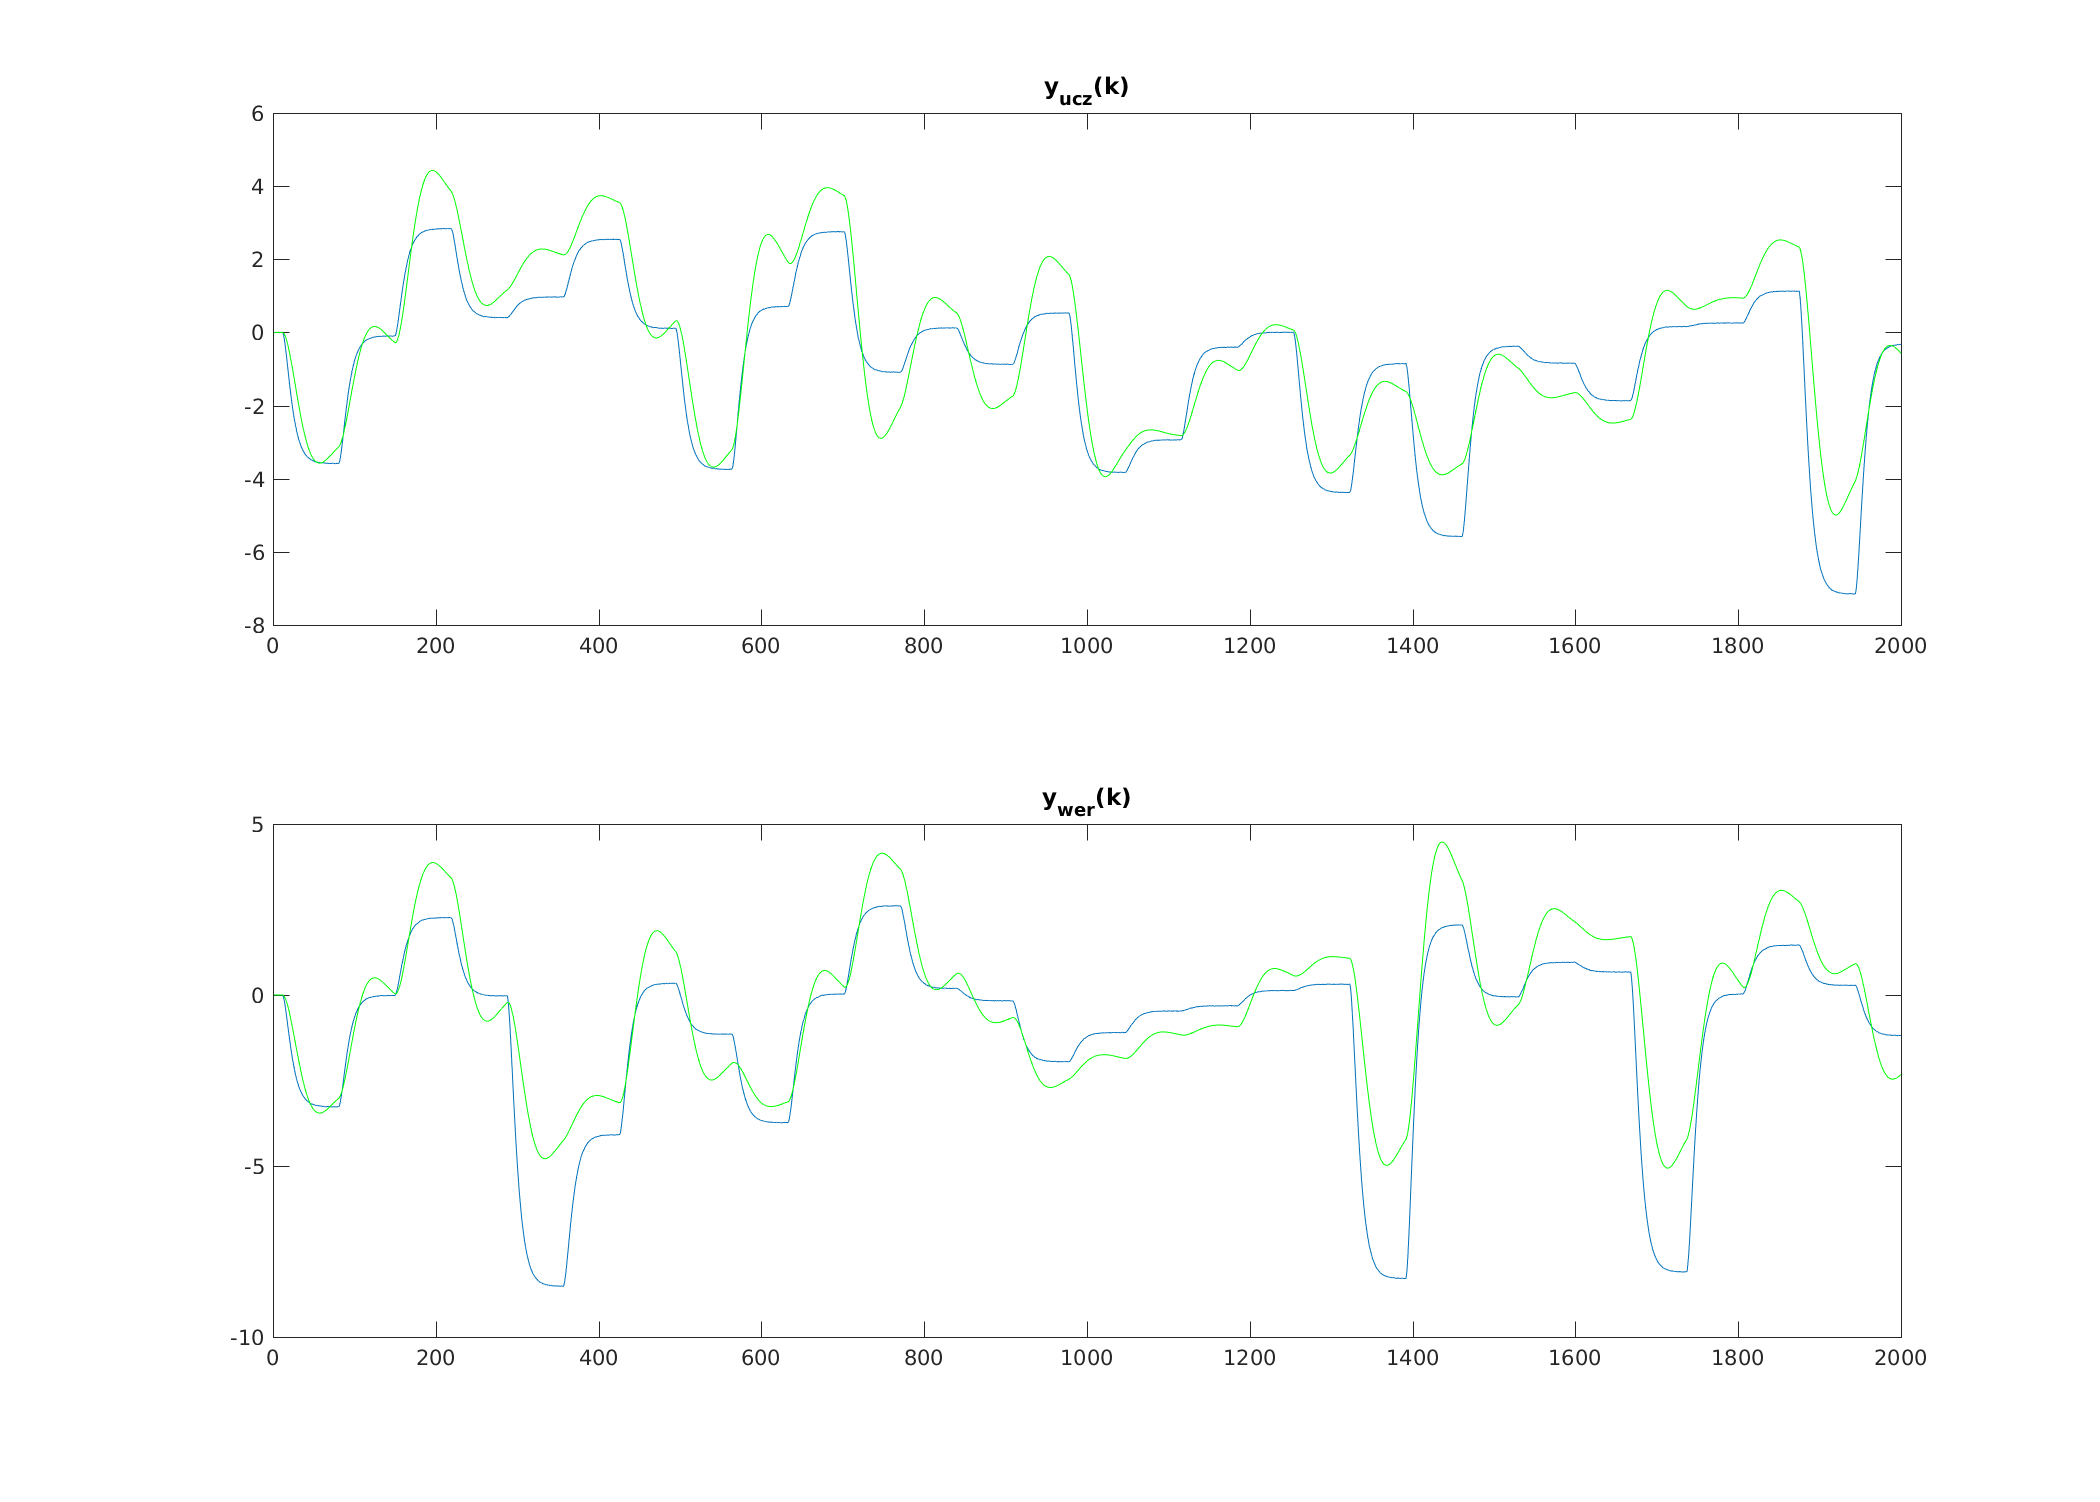
\includegraphics[scale=0.50]{dane_dyn_mod_rek_D_2.png}
\caption{Model z drugim rzędem dynamiki w trybie z rekurencją }
\label{}
\end{figure}

\subsubsection{Rzędu trzeciego}
Dla trzeciego rzędu dynamiki wielomian pierwszego stopnia ma postać : 
$$y(k) = b_1u(k-1)+b_2u(k-2)+b_3u(k-3) + a_1y(k-1)+a_2y(k-2)+a_3y(k-3)$$
\begin{figure}[H]
\centering
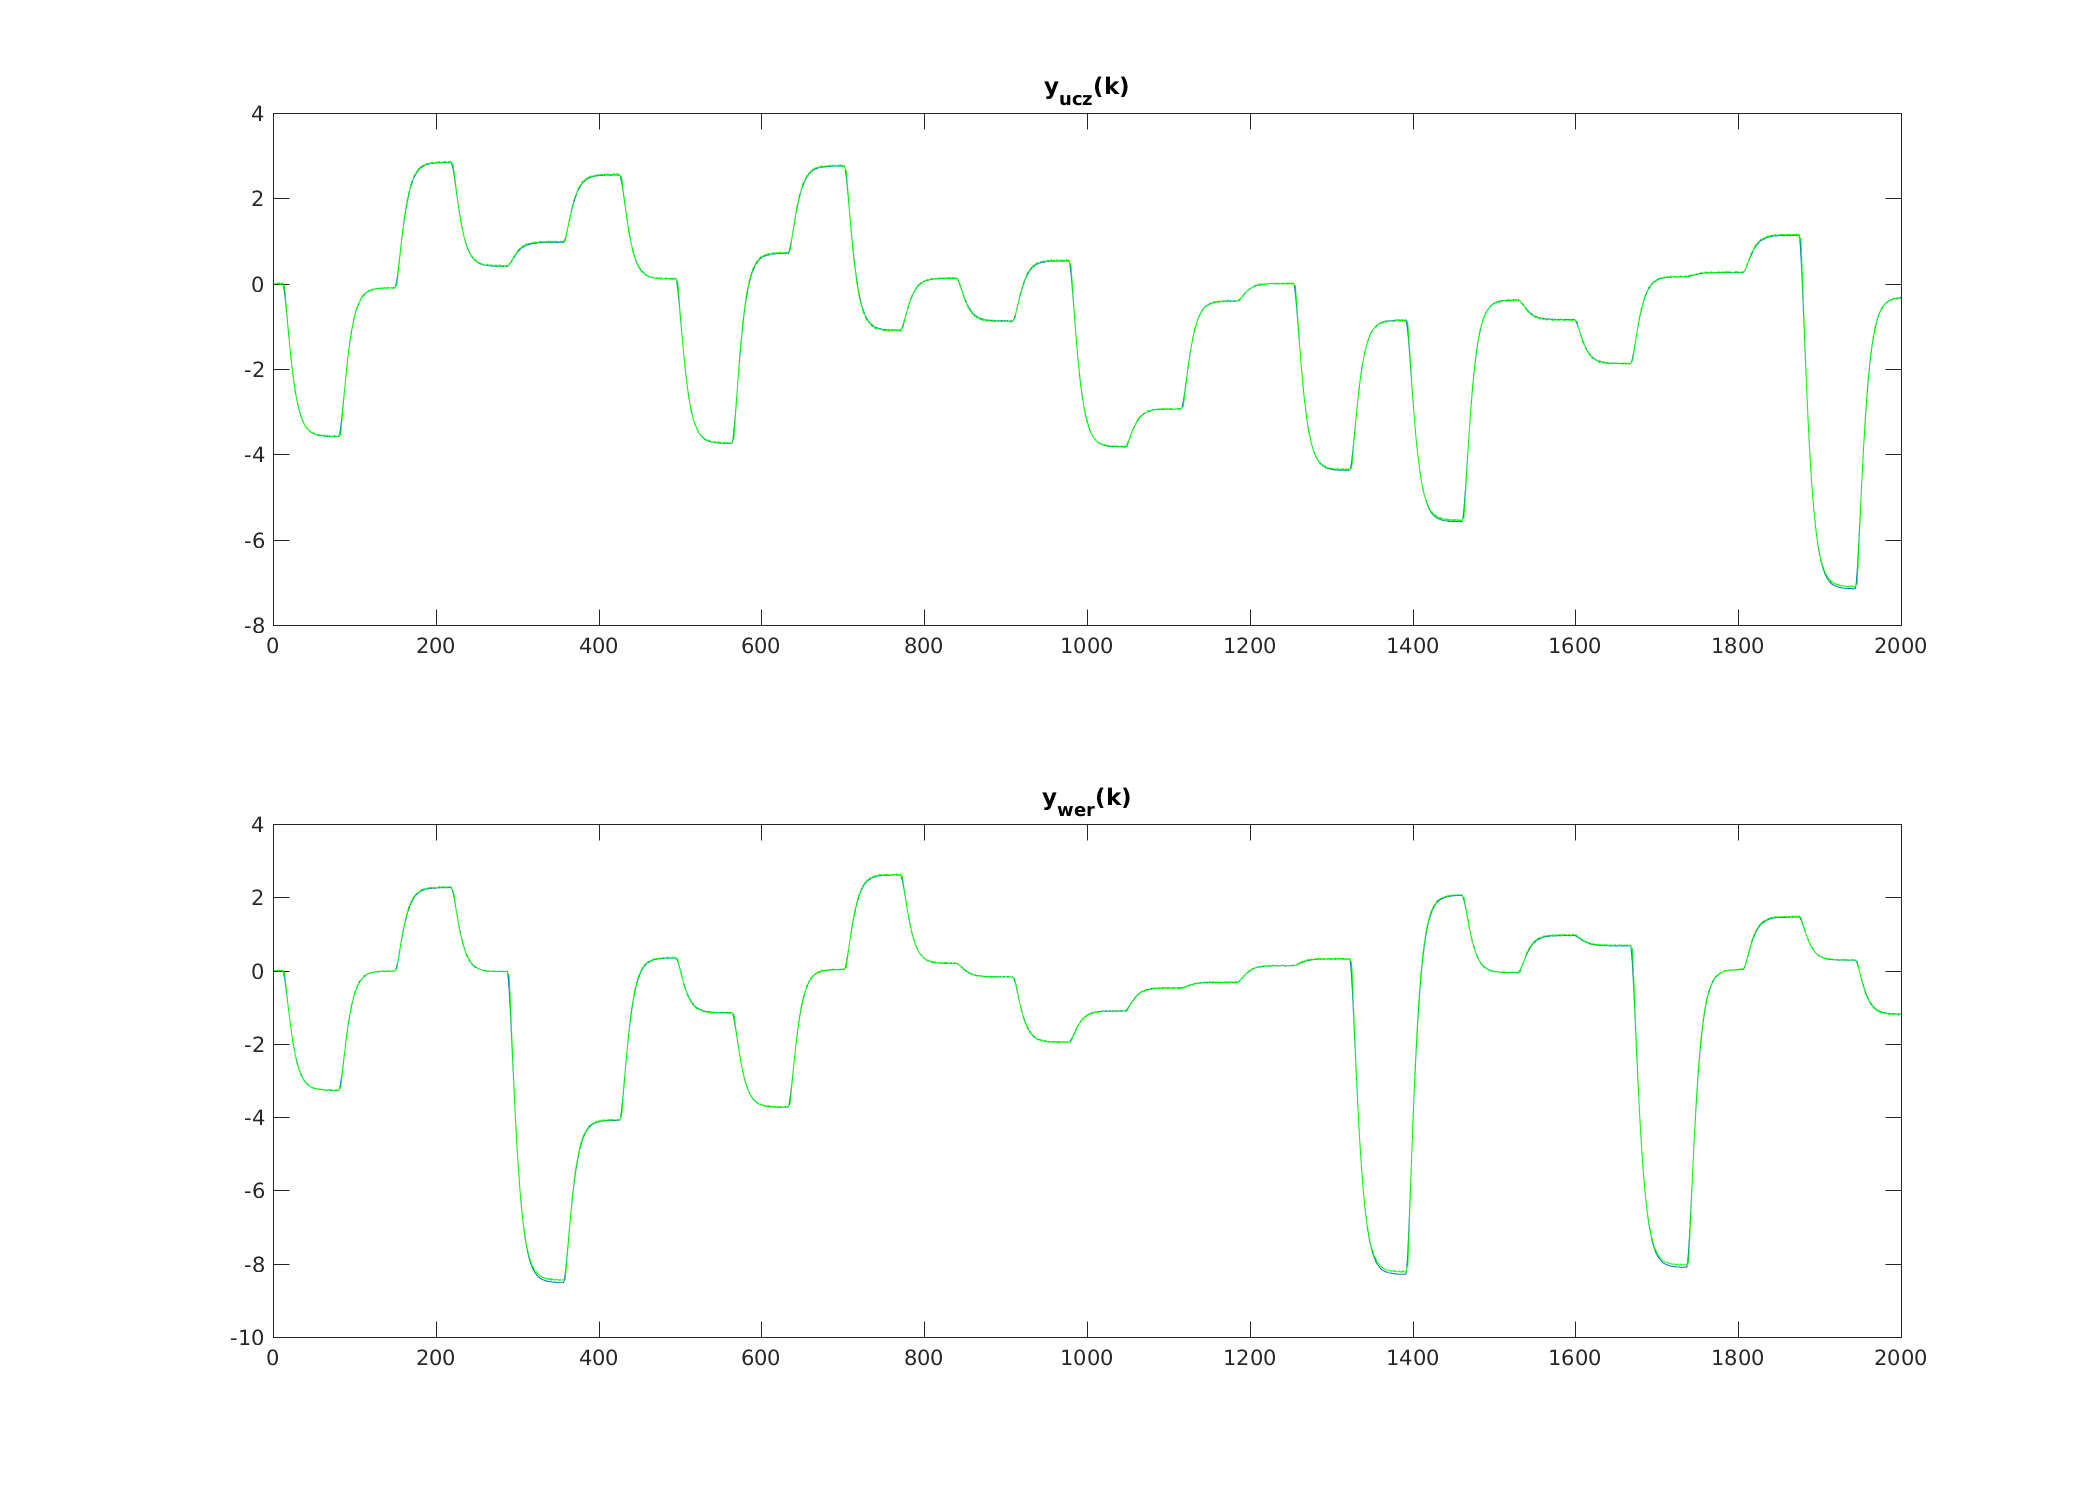
\includegraphics[scale=0.50]{dane_dyn_mod_brek_D_3.png}
\caption{Model z trzecim rzędem dynamiki w trybie bez rekurencji }
\label{}
\end{figure}
\begin{figure}[H]
\centering
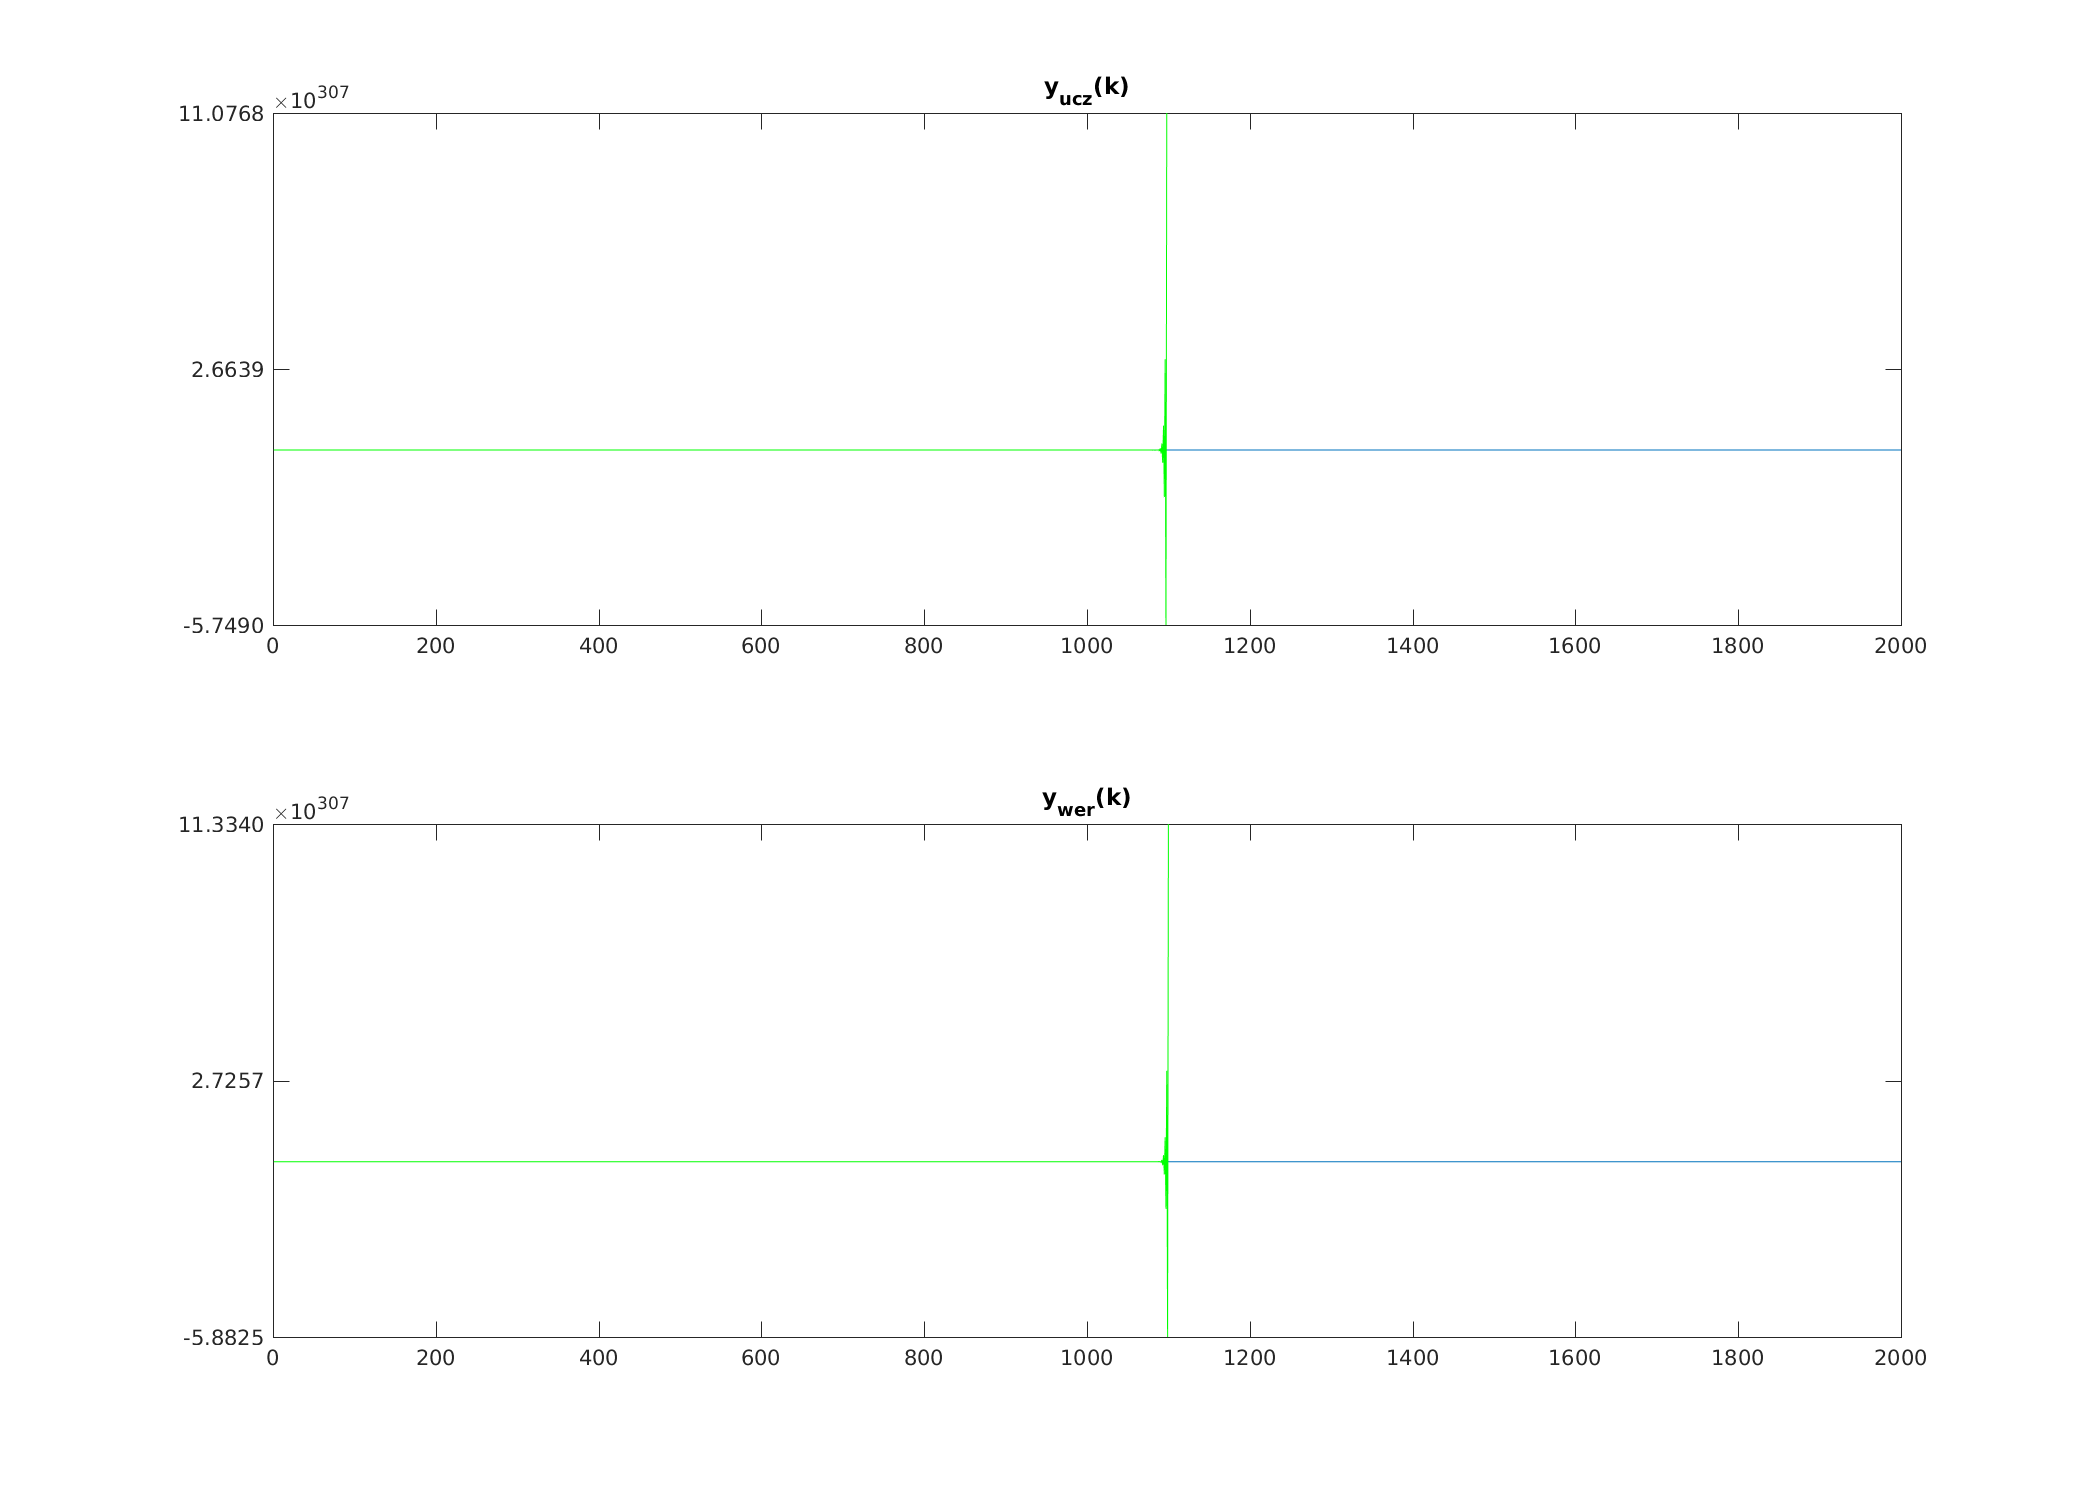
\includegraphics[scale=0.50]{dane_dyn_mod_rek_D_3.png}
\caption{Model z trzecim rzędem dynamiki w trybie z rekurencją }
\label{}
\end{figure}

\subsubsection{Porównanie modeli dynamicznych}
W celu podsumowania błędów modeli o różnych rzędach dynamiki została utworzona tabela: 
% Please add the following required packages to your document preamble:
% \usepackage{multirow}
\begin{table}[H]
\centering
\caption{Błedy dla modeli będących wielomianem stopnia pierwszego o różnych rzędach dynamiki}
\label{my-label}
\begin{tabular}{|c|l|l|l|l|}
\hline
\multirow{2}{*}{Rząd dynamiki} & \multicolumn{2}{l|}{Zbiór uczący} & \multicolumn{2}{l|}{Zbiór weryfikujący} \\ \cline{2-5} 
                               & Bez rekurencji   & Z rekurencją   & Bez rekurencji      & Z rekurencją      \\ \hline
1                              & 8.345317e+00     & 3.337650e+03   & 1.360255e+01        & 5.609383e+03      \\ \hline
2                              & 3.635287e-01     & 1.035374e+04   & 5.944462e-01        & 1.497991e+04      \\ \hline
3                              & 9.529738e-02     & 1.001853e+04   & 9.520603e-02        & 1.417891e+04      \\ \hline
\end{tabular}
\end{table}


\subsection{Wybór najlepszego modelu}
\subsection{Modele dynamiczne wyznaczane metodą najmniejszych kwadratów} 
\subsubsection{Modele o dynamice pierwszego rzędu}
\subsubsection{Modele o dynamice drugiego rzędu}
\subsubsection{Modele o dynamice trzeciego rzędu}
\subsubsection{Porównanie modeli} %tabelka
\subsection{Wybór najlepszego modelu nieliniowego}


\section{Wyznaczanie statycznego modelu nieliniowego}
\subsection{Statyczny model nieliniowy}
\subsection{Reprezentacja graficzna statycznego modelu nieliniowego}



\end{document}